\documentclass[10pt,aspectratio=169]{beamer}

\usetheme[progressbar=frametitle]{metropolis}
\setsansfont{Roboto Light}
\usepackage{appendixnumberbeamer}
\usepackage{booktabs}
\usepackage[scale=2]{ccicons}
\usepackage{pgfplots}
\usepgfplotslibrary{dateplot}
\usepackage{tabularx}
\usepackage[absolute,overlay]{textpos}
\usepackage{xspace}
\usepackage{fontawesome}
% \usepackage{fontawesome5}
\newcommand{\themename}{\textbf{\textsc{metropolis}}\xspace}
\usepackage{pgfpages}	
\usepackage{array} 
\usepackage{graphicx,multirow}
\usepackage{tikz}
\usetikzlibrary{arrows.meta,
                chains,
                positioning}
\usepackage{graphbox}
\usepackage{mathabx}
\usepackage{pgfgantt}
\usepackage{textpos} 

% \setbeameroption{show notes on second screen=right} % Both
\setbeameroption{hide notes} % Only slides


% \title{Constraining and forecasting the impact and recovery of vegetation from natural hazards}
\title{Volcanic hazard assessment -- Day 2: Tephra fallout}
\subtitle{\normalsize Volcanic risk module / CERG--C / ELSTE}
\date{\vspace*{.5em} \footnotesize Costanza Bonadonna, Lucia Dominguez, Corine Frischknecht, Eduardo Rossi, Maria-Paz Reyes}
\author{\textbf{Sébastien Biasse} - sebastien.biasse@unige.ch}
\institute{11 May 2022}

\begin{document}

\maketitle 

\begin{frame}[standout]
  \alert{Good morning!}\\ \vspace*{0.5em}
  \textnormal{
  $\rightarrow$ Download and save Day 2 material \alert{onto your H: drive}\\ \vspace*{0.5em}
  $\rightarrow$ \alert{Extract} content (i.e., right click, \textit{"Extraire tout..."})\\ \vspace*{0.5em}
  $\rightarrow$ \alert{Extract} the content of \alert{TephraProb.zip} (yes --- still on the H: drive)\\ \vspace*{0.5em}
  $\rightarrow$ Try and open \alert{Matlab 2022a}\\
  }
\end{frame}


\begin{frame}{What is tephra?}
  \only<1>{ 
    \centering Fragmented material regardless of size or composition \\ \vspace*{1em}
    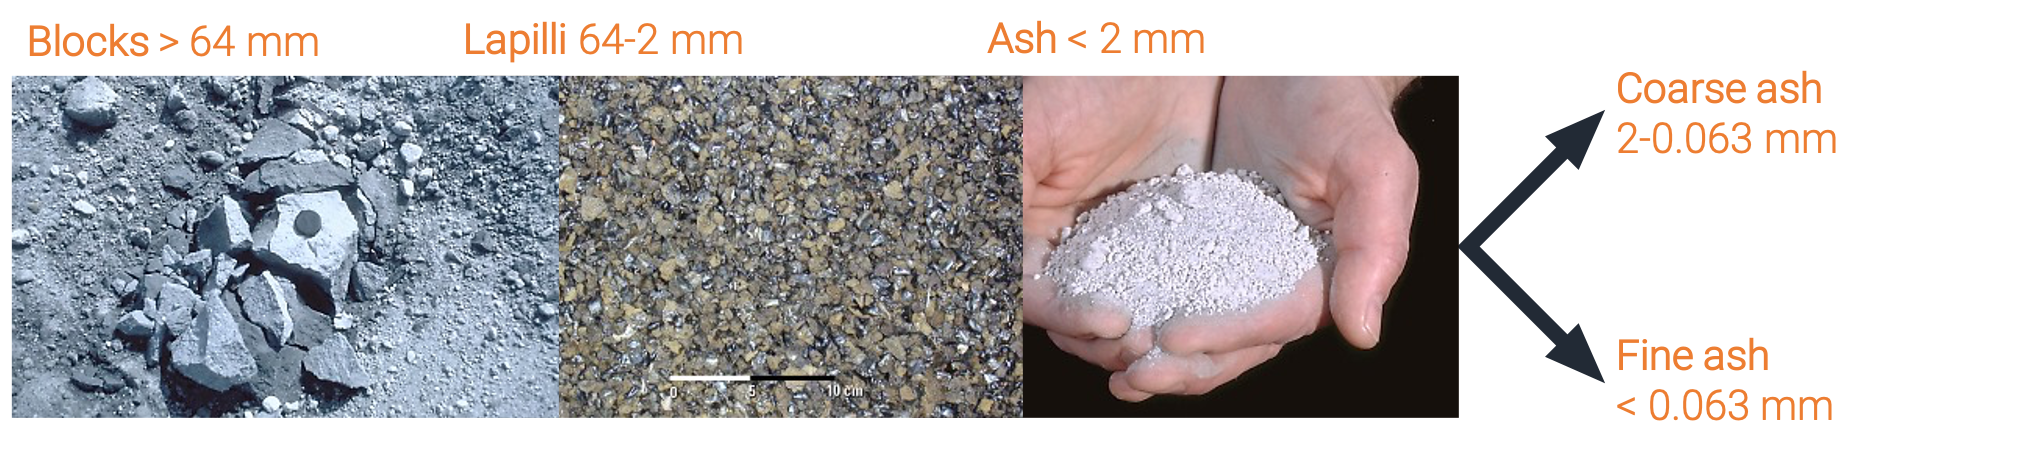
\includegraphics[width=1\textwidth]{img/tephra_def.png}
  }
  \only<2>{ 
    \begin{columns}[T]
      \begin{column}{0.5\textwidth}	
        \textbf{Pyroclastic density currents (PDC)} \\ \vspace*{1em}
        \centering 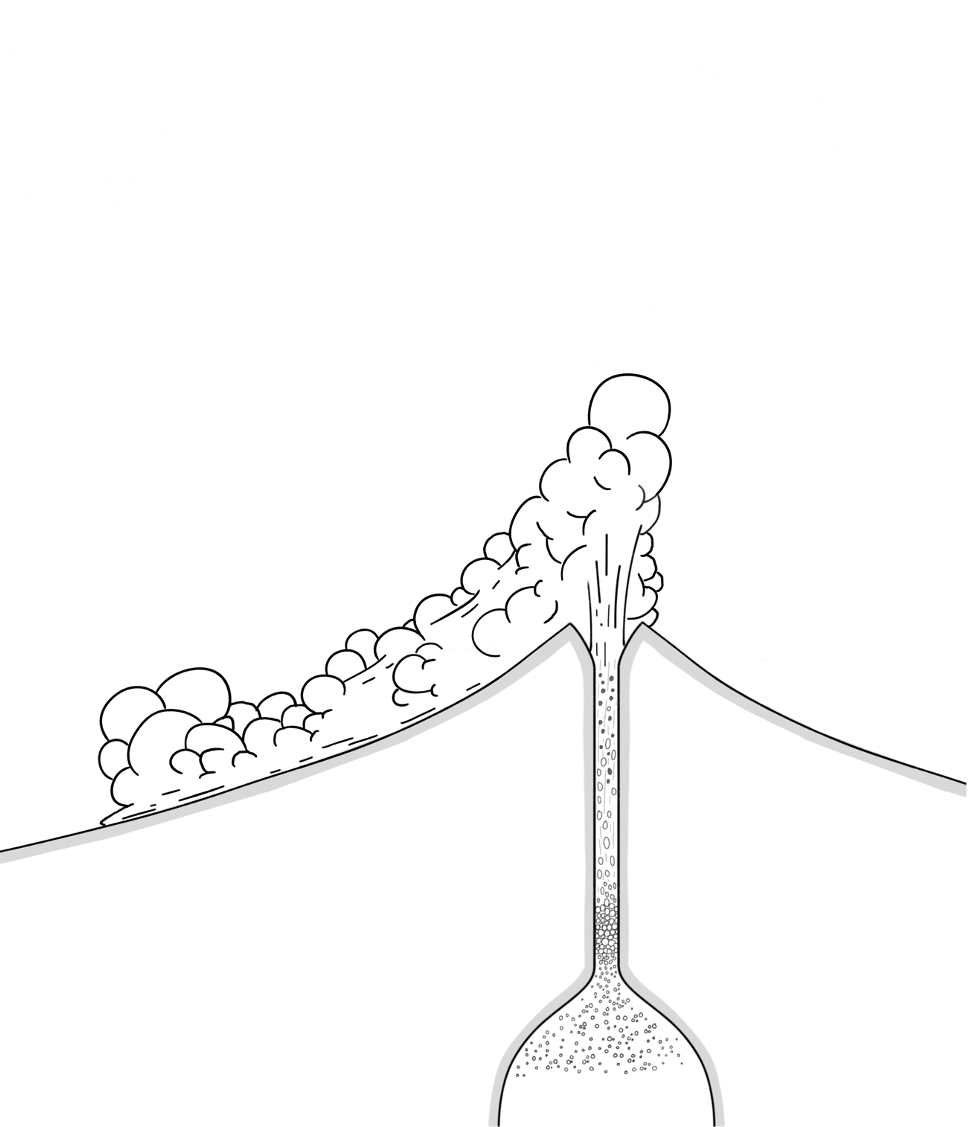
\includegraphics[width=.85\textwidth]{img/tephra_flow.png}
      \end{column}

      \begin{column}{0.5\textwidth}	
        \textbf{Tephra fall} \\ \vspace*{1em}
        \centering 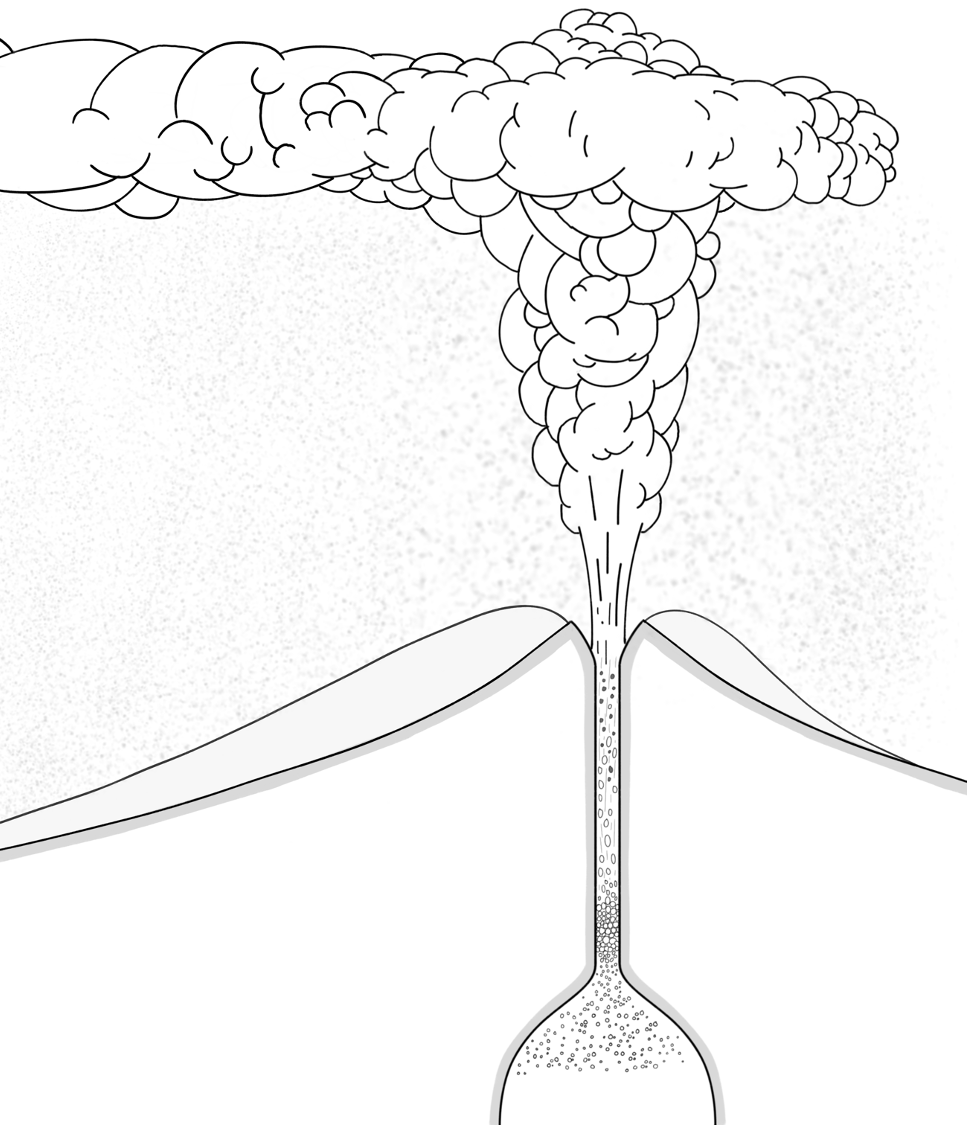
\includegraphics[width=.85\textwidth]{img/tephra_fall.png}
      \end{column}
    \end{columns}
  }
\end{frame}


\begin{frame}[t]{Why are tephra deposits important?}
  \only<1>{ 
    \centering $\rightarrow$ They record \alert{eruption dynamics} \\ \vspace*{1em}
    \includegraphics[width=.85\textwidth]{../docs/img/tephra/strati.png}
  }
  \only<2>{ 
    \centering $\rightarrow$ They record \alert{eruption dynamics} \\ \vspace*{1em}
    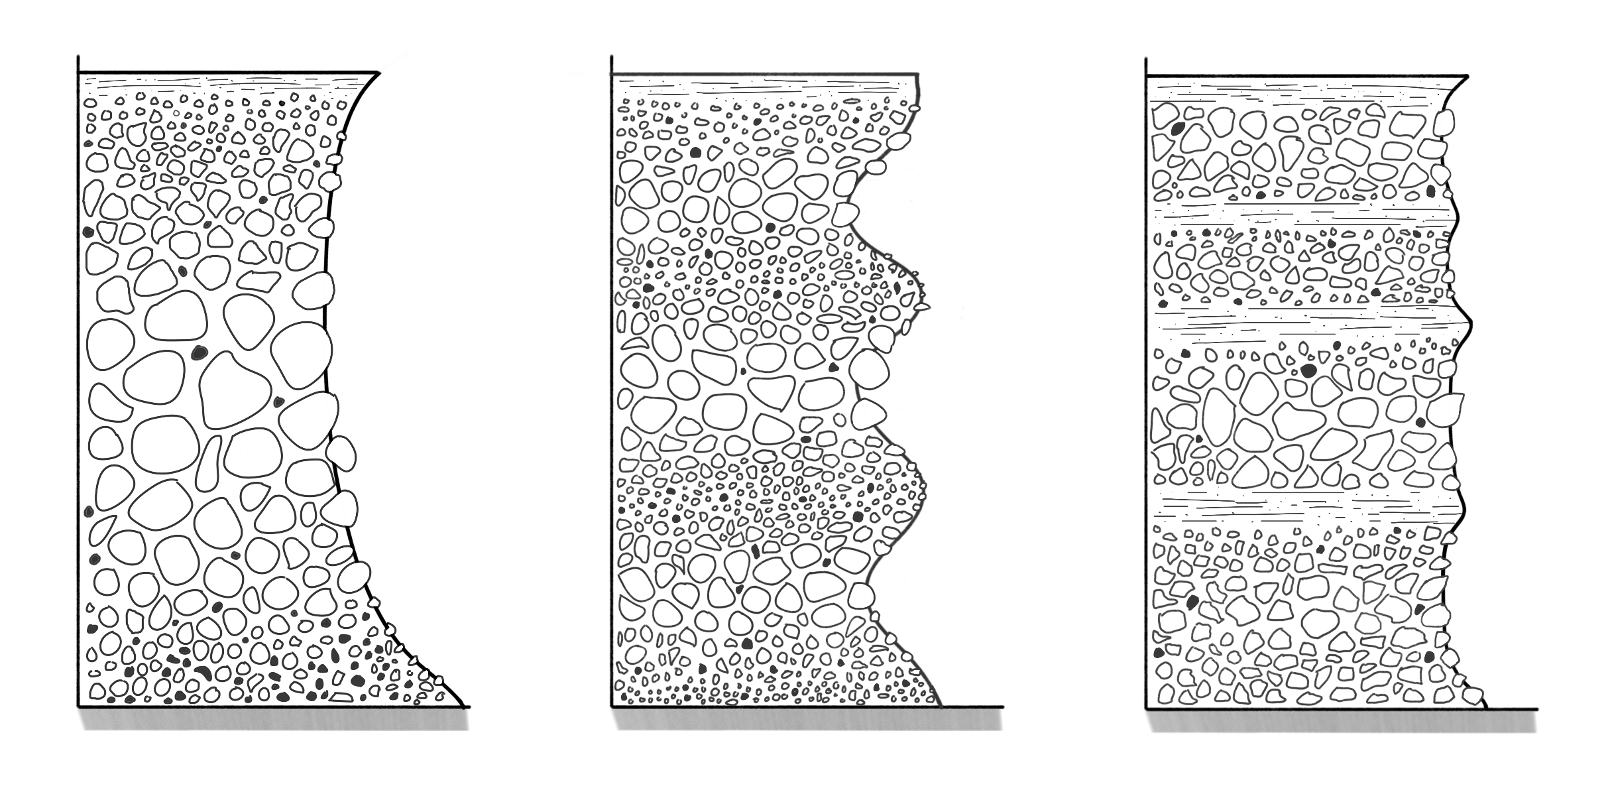
\includegraphics[width=1\textwidth]{img/outrcrops_drawing.png}
  }
  \only<3>{ 
    \centering $\rightarrow$ They are a \alert{time machine} to past eruptions \\ \vspace*{1em}
    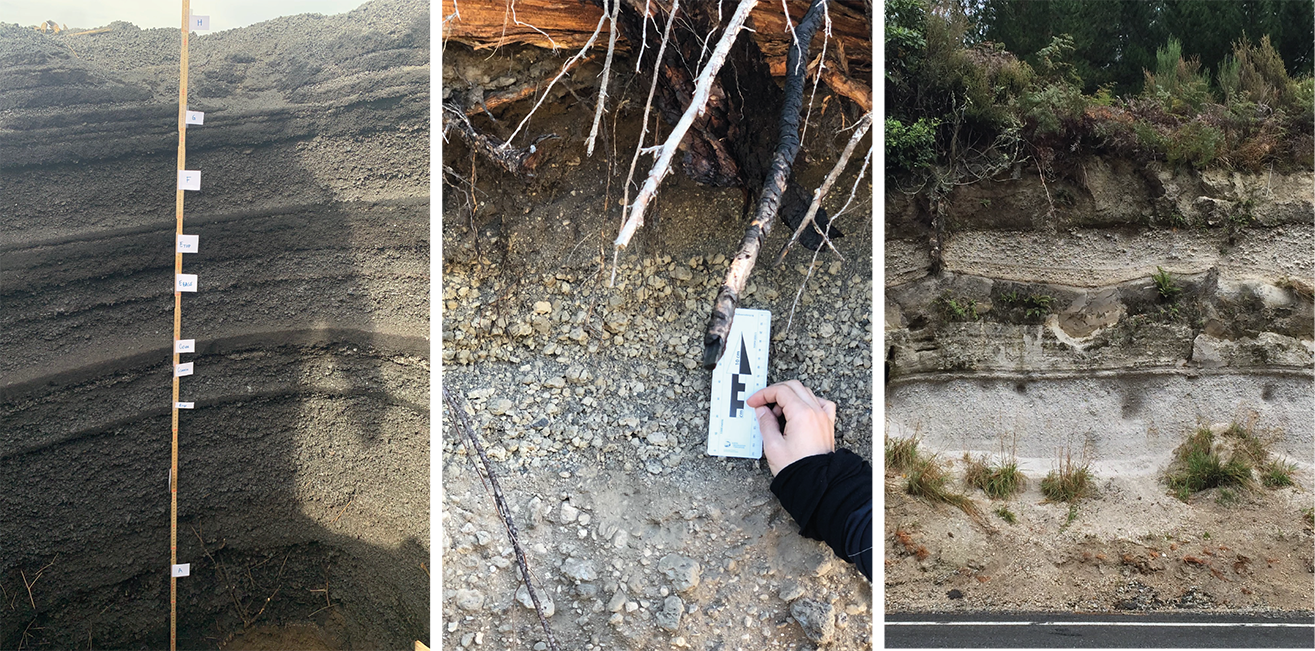
\includegraphics[width=1\textwidth]{img/outcrops_examples.png}
  }
  \only<4>{ 
    \centering $\rightarrow$ They allow quantifying \alert{eruption source parameters} \\ \vspace*{1em}
    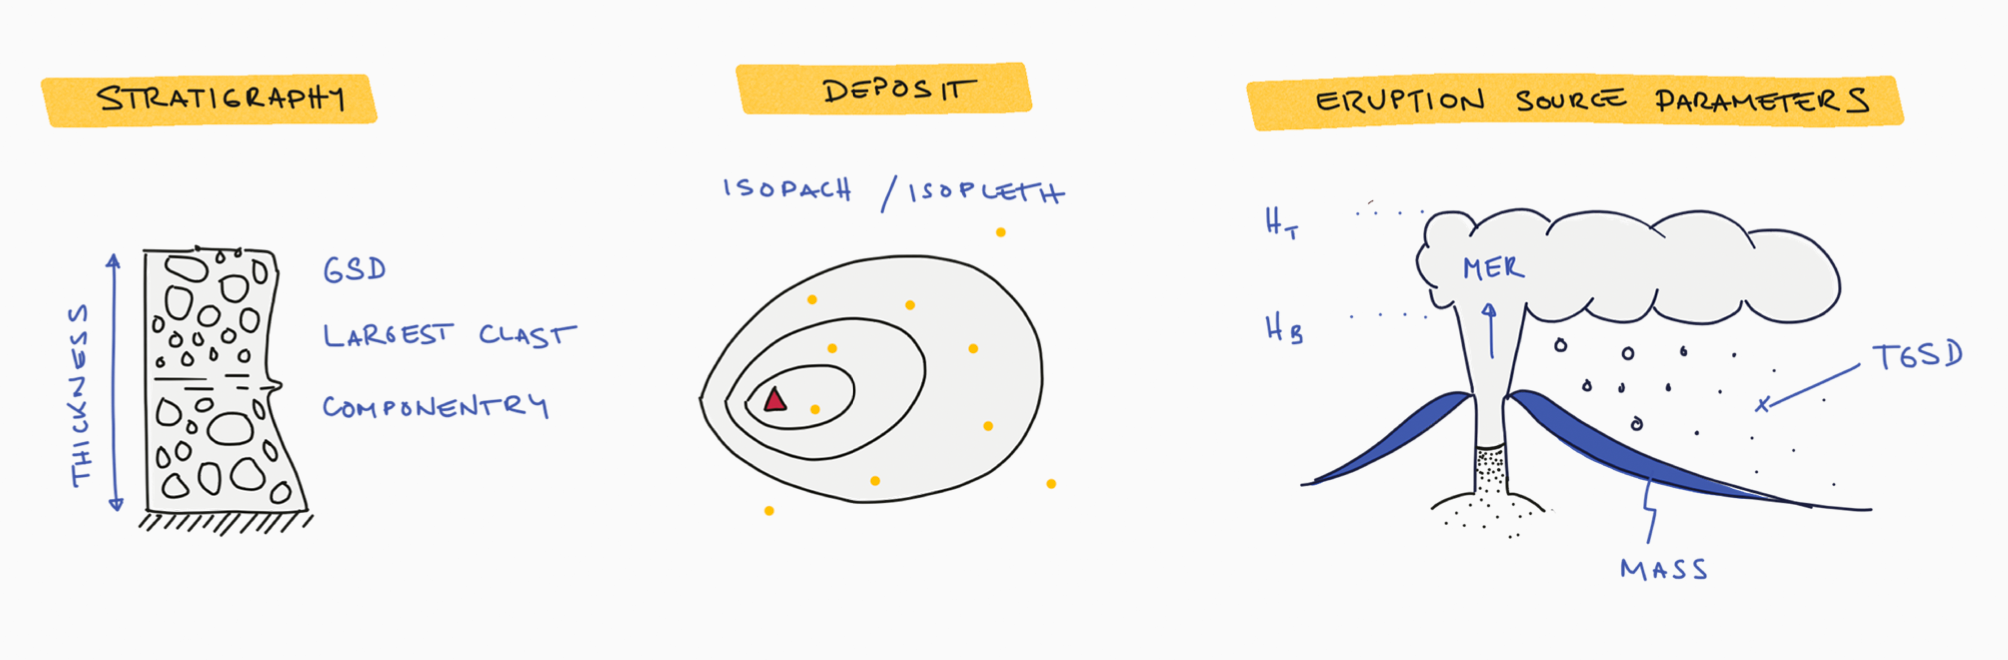
\includegraphics[width=1\textwidth]{img/field_characterisation.png}
    \centering $\rightarrow$ Plume height, erupted mass, total grain-size distribution \\ \vspace*{1em}
  }
  \only<5>{ 
    \begin{columns}[T]
      \begin{column}{0.6\textwidth}	
        Mapping toolbox \\ \vspace*{1em}
        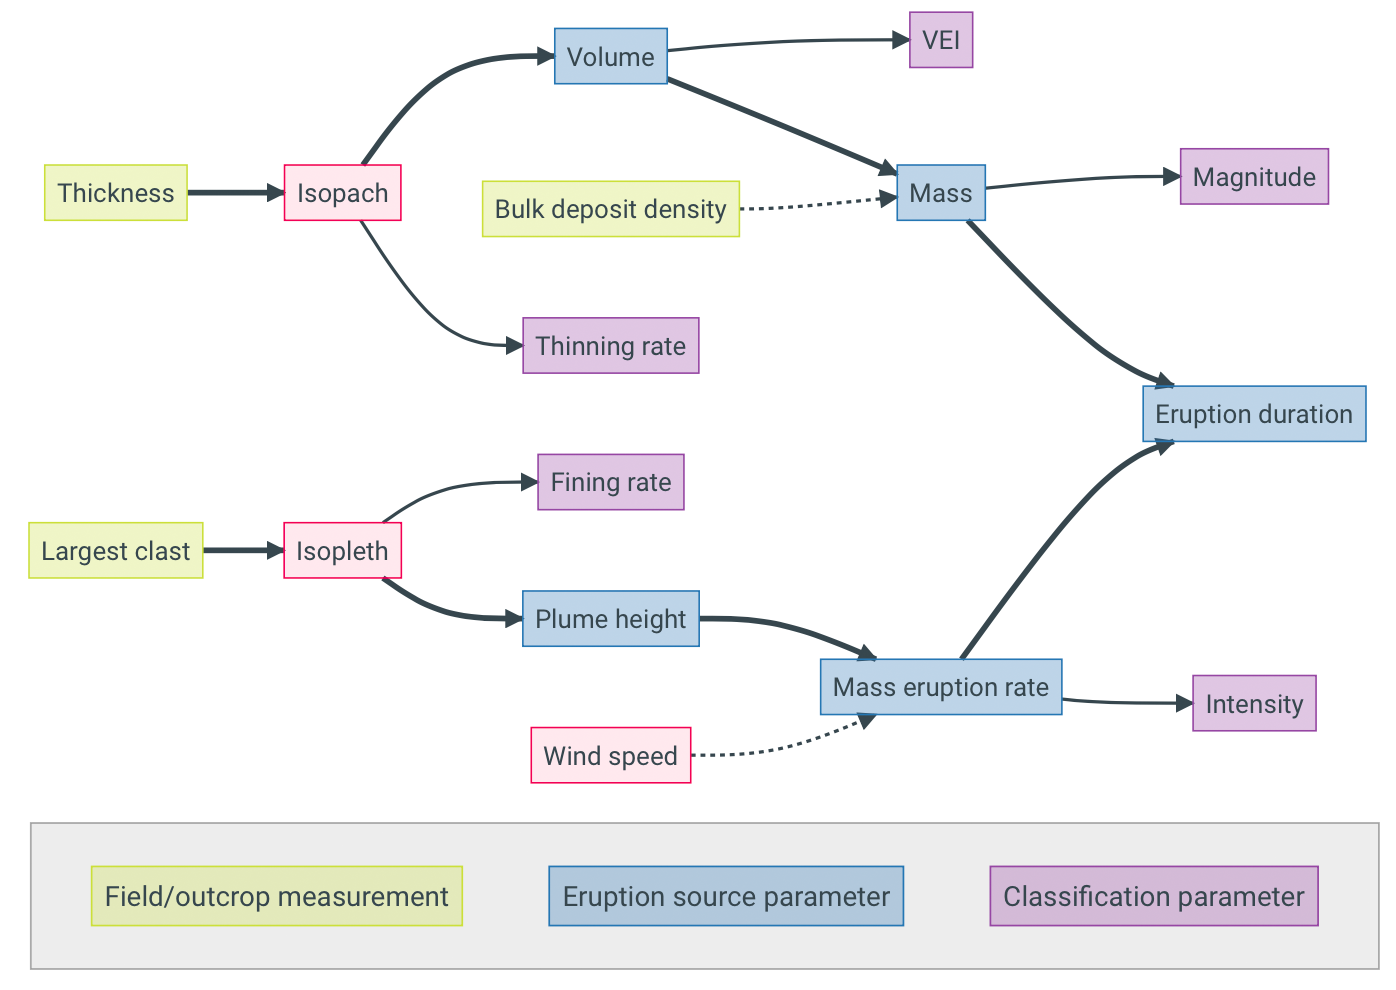
\includegraphics[width=1\textwidth]{img/toolbox.png}
      \end{column}
      \begin{column}{0.4\textwidth}	
        Volcanic Explosivity Index (VEI) \\ \vspace*{1em}
        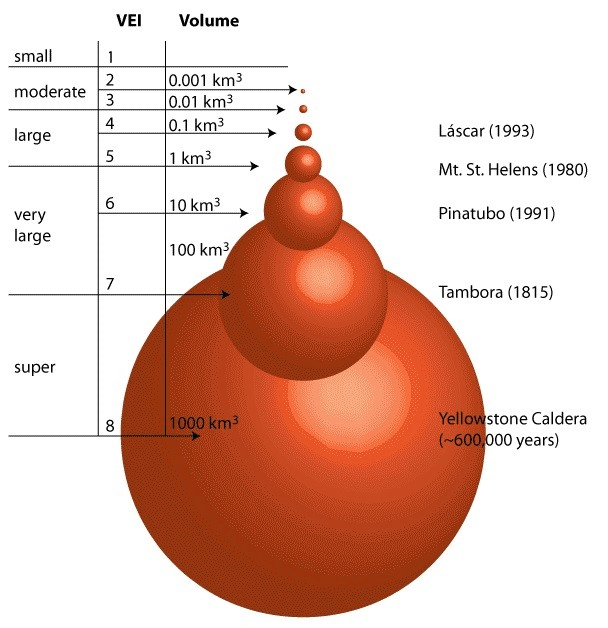
\includegraphics[width=1\textwidth]{../docs/img/tephra/vei.png}
      \end{column}
    \end{columns}
  }
  \only<6>{ 
    \begin{columns}[T]
      \begin{column}{0.6\textwidth}	
        Magnitude vs. intensity \\ \vspace*{1em}
        \centering 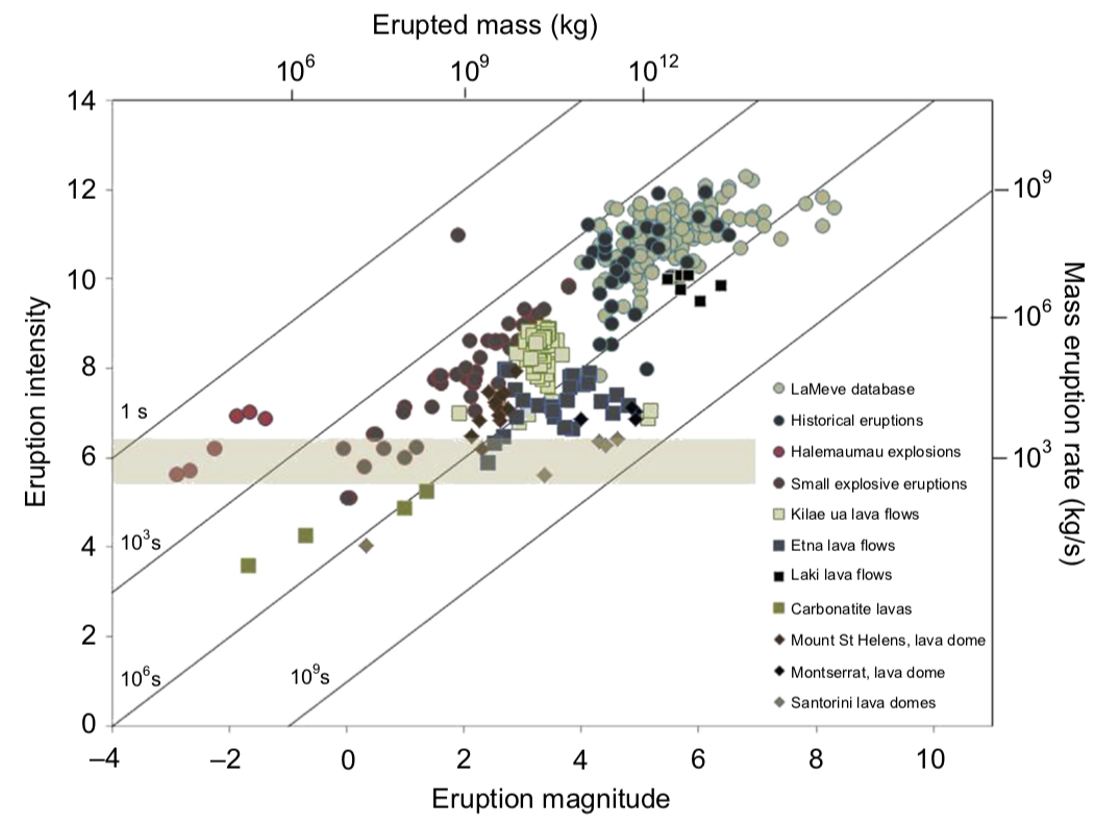
\includegraphics[width=.8\textwidth]{img/intensity.png}\\

        \alert{Intensity}: $log_{10}(MER\ [kg/m^{2}])+3$\\
        \alert{Magnitude}: $log_{10}(Mass\ [kg])+-7$\\

      \end{column}
      \begin{column}{0.4\textwidth}	
        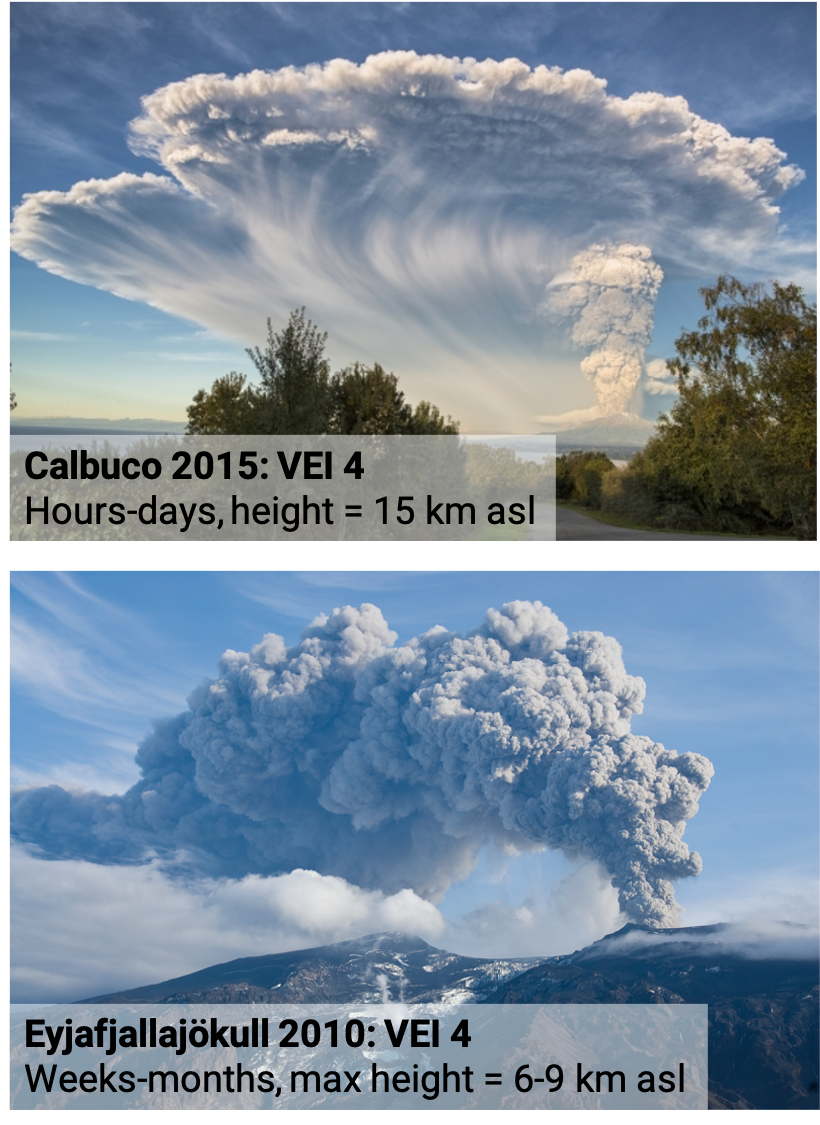
\includegraphics[width=.9\textwidth]{img/calbuco-eyja.png}
      \end{column}
    \end{columns}
  }
\end{frame}

\begin{frame}[standout]
  "The \alert{past} is the key to the \alert{future}"
\end{frame}


\begin{frame}[t]{Why are tephra deposits hazardous?}
  \only<1>{ 
    \centering Cited as a cause of death in 21\% of volcanic eruptions $\rightarrow$ \alert{roof collapse}    \\ \vspace*{1em}
    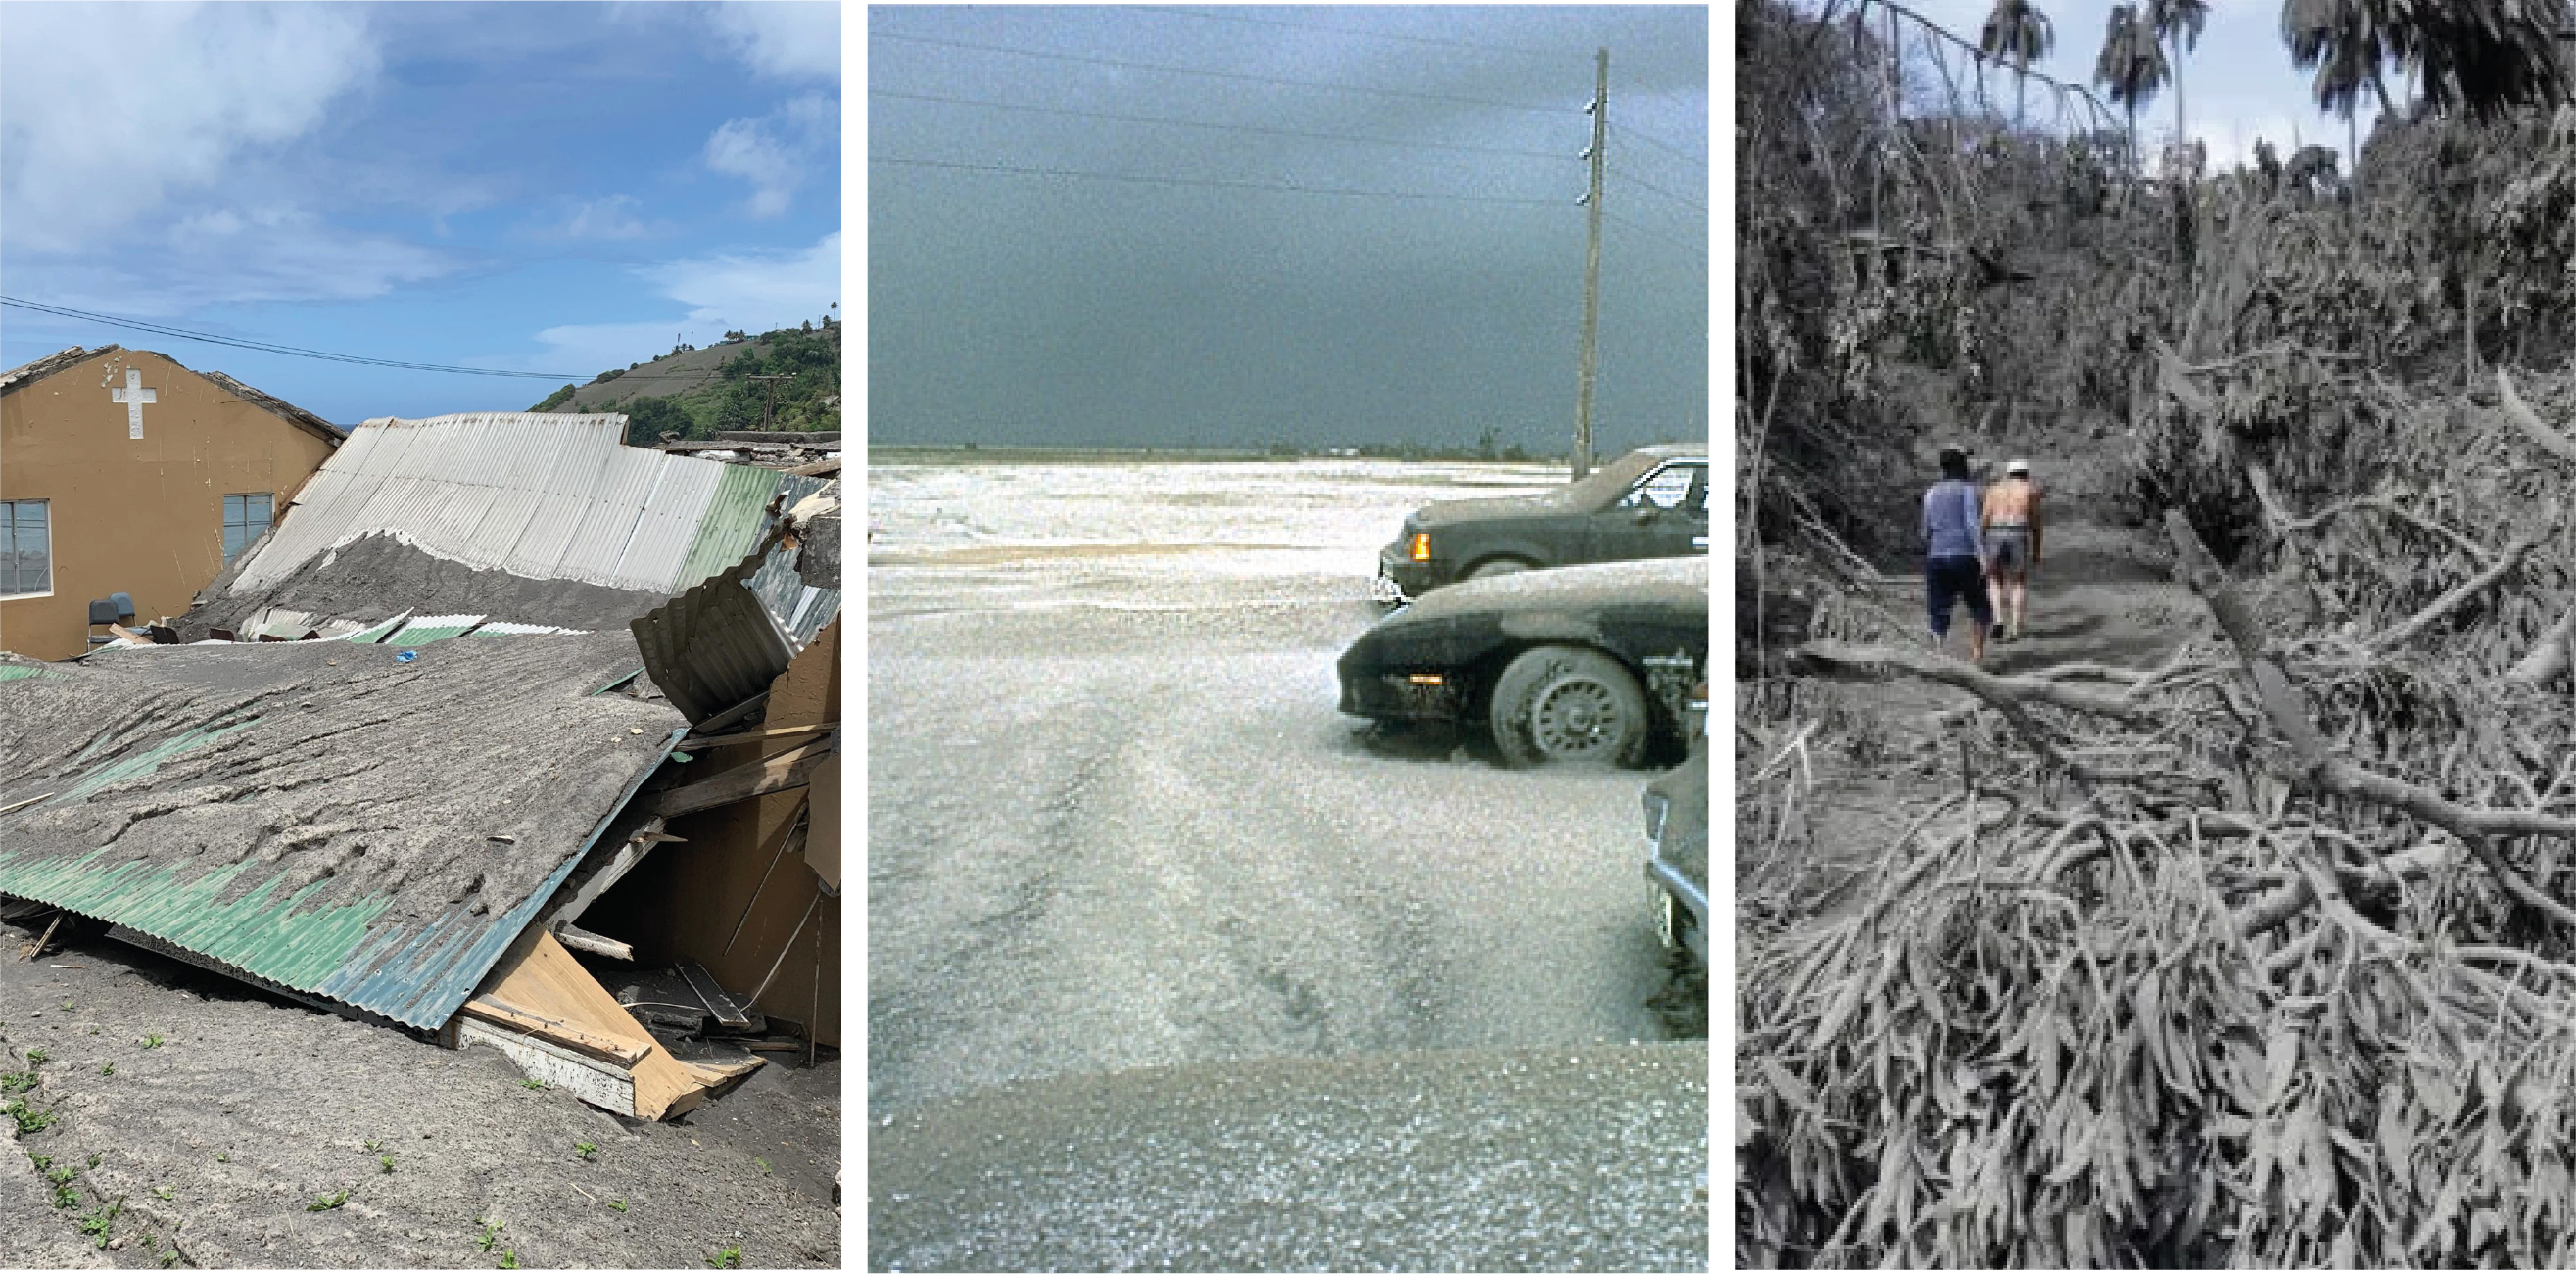
\includegraphics[width=1\textwidth]{img/tephra_impact.png}
  }
  \only<2>{ 
    \centering Complex \alert{spatio-temporal} impact patterns \\ 
    \centering Destruction $\rightarrow$ Damage $\rightarrow$ Disruption\vspace*{1em}
    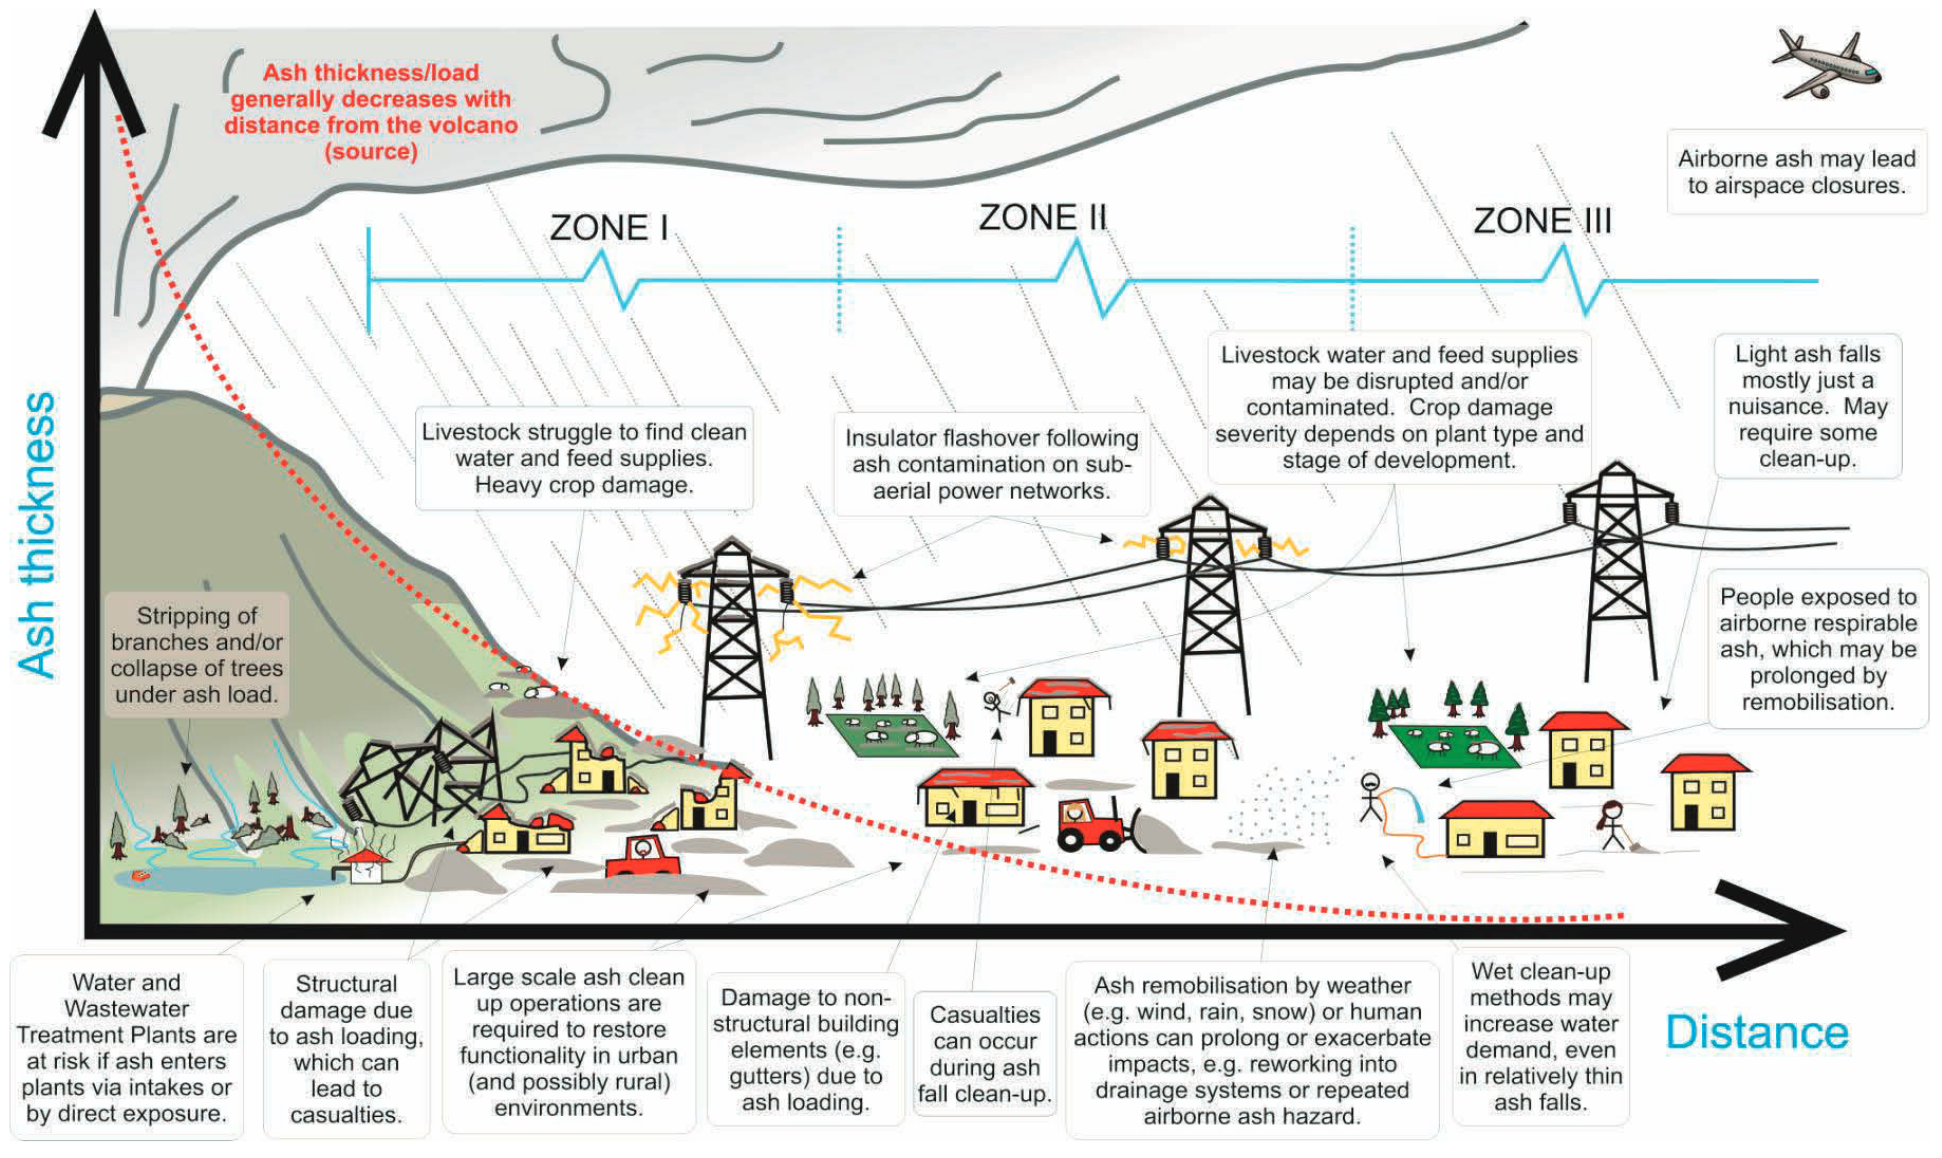
\includegraphics[width=.75\textwidth]{../docs/img/tephra/impact.png}
  }
\end{frame}

\begin{frame}[standout]
  "\alert{There is no such thing as a natural disaster} "\\
  \begin{flushright}
    --- UNDRR
  \end{flushright}
\end{frame}

\begin{frame}[t]{The interface between hazard and impact}
  \centering \LARGE $ I = f(H, V)$
  \normalsize
  
  \begin{itemize}
    \item \textbf{I:} Impact from \alert{ground tephra accumulation} 
    \item \textbf{H:} Spatio(-temporal) distribution of \alert{hazard intensity metrics}
    \item \textbf{V:} Vulnerability $\rightarrow$ how exposed element will be \alert{negatively impacted} by hazard
  \end{itemize} \vspace*{1.5em}

  \only<2>{ 
    \begin{columns}[T]
      \begin{column}{0.3\textwidth}	
          \textbf{Damage/disruption states (DDS)}: Stepwise categorisation of impact as a function of hazard intensity
      \end{column}
      \begin{column}{0.7\textwidth}	
        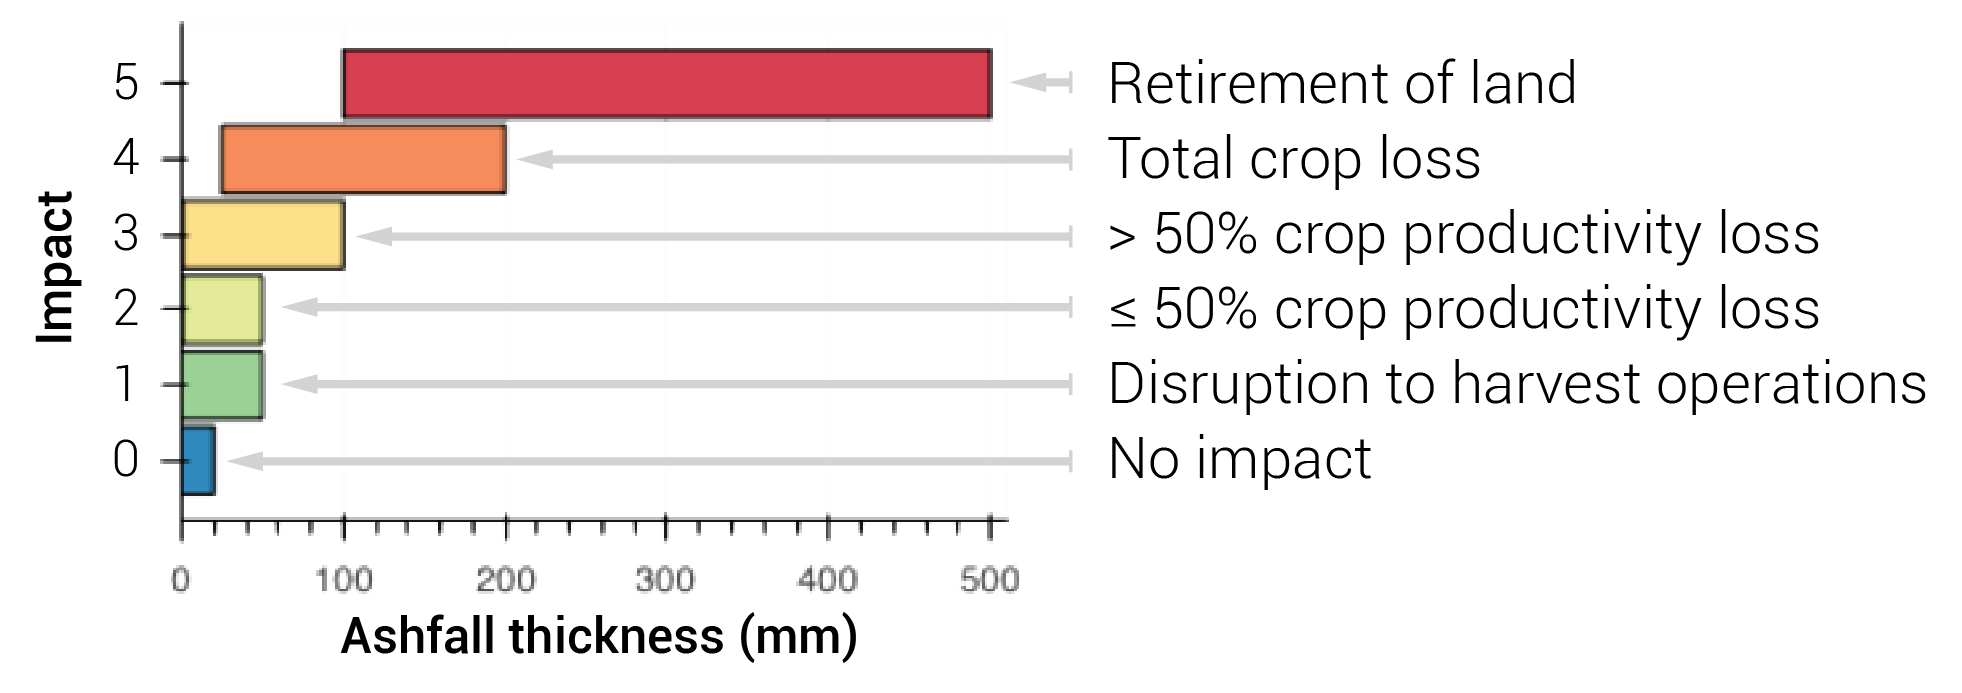
\includegraphics[width=1\textwidth]{../docs/img/dds.png}
      \end{column}
    \end{columns}
  }

  \only<3>{ 
    \begin{columns}[T]
      \begin{column}{0.3\textwidth}	
          \textbf{Fragility/Vulnerability functions}: Mathematical function expressing a probability of impact/relative cost for a given hazard intensity
      \end{column}
      \begin{column}{0.7\textwidth}	
       \centering 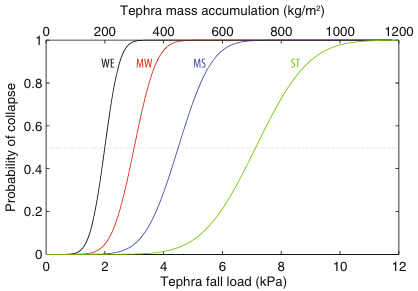
\includegraphics[width=.67\textwidth]{../docs/img/tephra/fragility.png}
      \end{column}
    \end{columns}
  }

  \only<4->{
    \textbf{The complexity of volcanic risk}
    \begin{itemize}
      \item<4- | alert@4> \textbf{Multi--hazard} $\rightarrow$ interaction \& variability in space and time
      \item<5- | alert@5> Wide range of \textbf{eruptive styles} $\rightarrow$ no magnitude/intensity relationship
      \item<6- | alert@6> Multiple \textbf{hazard metrics} $\rightarrow$ Tephra: load, thickness, grain-size, soluble salts
    \end{itemize}
  }

\end{frame}


\begin{frame}[standout]
  Pre--event exposure/impact/risk studies require:\\ \vspace*{1em}
  $\rightarrow$ \textnormal{Ability to \textit{predict} the hazard}
\end{frame}

\section{\alert{Tephra fallout part I} \\ Physical modeling}

\begin{frame}{What is a model?}

  \begin{columns}[T]
    \begin{column}{0.7\textwidth}	
      \vspace*{1em}
      \textbf{Models are approximation of reality!} \vspace*{1em}
      \begin{itemize}
        \item<1- |alert @ 1> For natural hazards:
        \begin{itemize}
          \item Initial conditions $\rightarrow$ \alert{MODEL} $\rightarrow$ Hazard intensity
        \end{itemize}
      \end{itemize}

      \only<2>{
        \vspace*{1.5em}
        \textbf{Type of models:} \vspace*{1em}
        \begin{itemize}
          \item<2- |alert @ 2> \textbf{Mathematical}: Data-driven, include statistical or machine learning-powered models
          \item<2- |alert @ 2> \textbf{Physical}: rely on a simplified formulation of physical laws

        \end{itemize}
      }
    \end{column}

    \begin{column}{0.3\textwidth}	
      \centering 
\includegraphics[width=.85\textwidth]{img/model.png}
    \end{column}
  \end{columns}
  
\end{frame}



\begin{frame}{Model parametrisation for tephra fallout}
  \only<1>{
    \textbf{1. The rise of magma to the surface} \\ 
    \begin{flushright}
      \vspace*{-1em}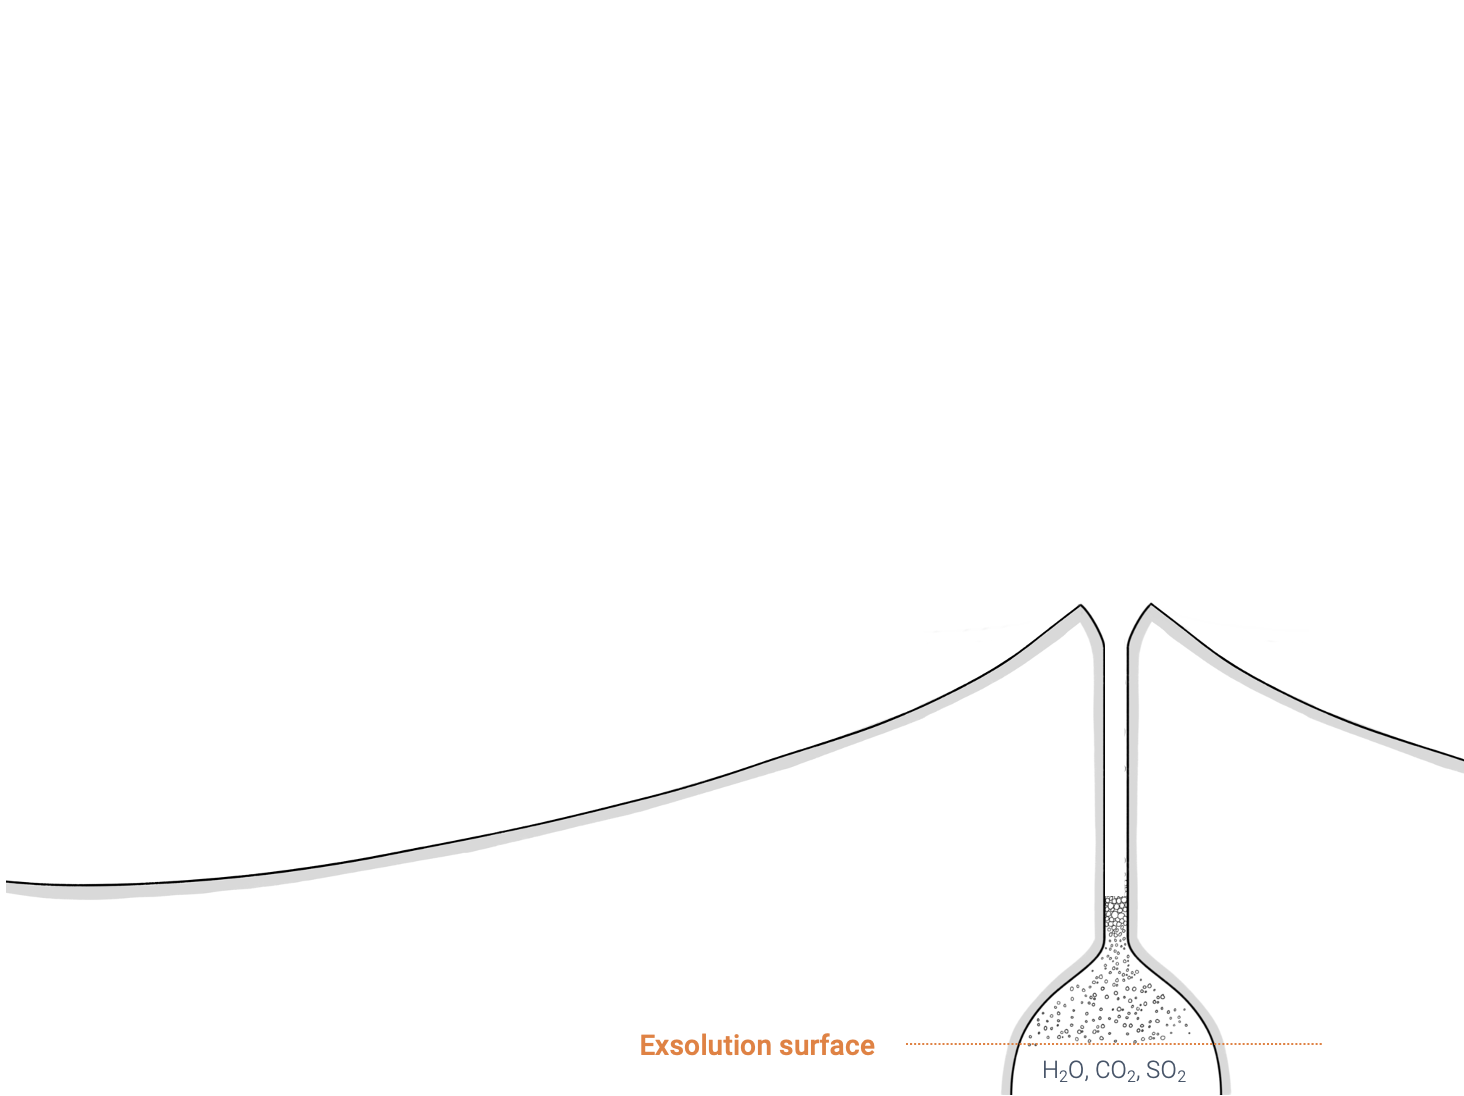
\includegraphics[width=.7\textwidth]{../docs/img/model/m1.png}
    \end{flushright}
  }
  \only<2>{
    \textbf{2. The generation of tephra} \\ 
    \begin{flushright}
      \vspace*{-1em}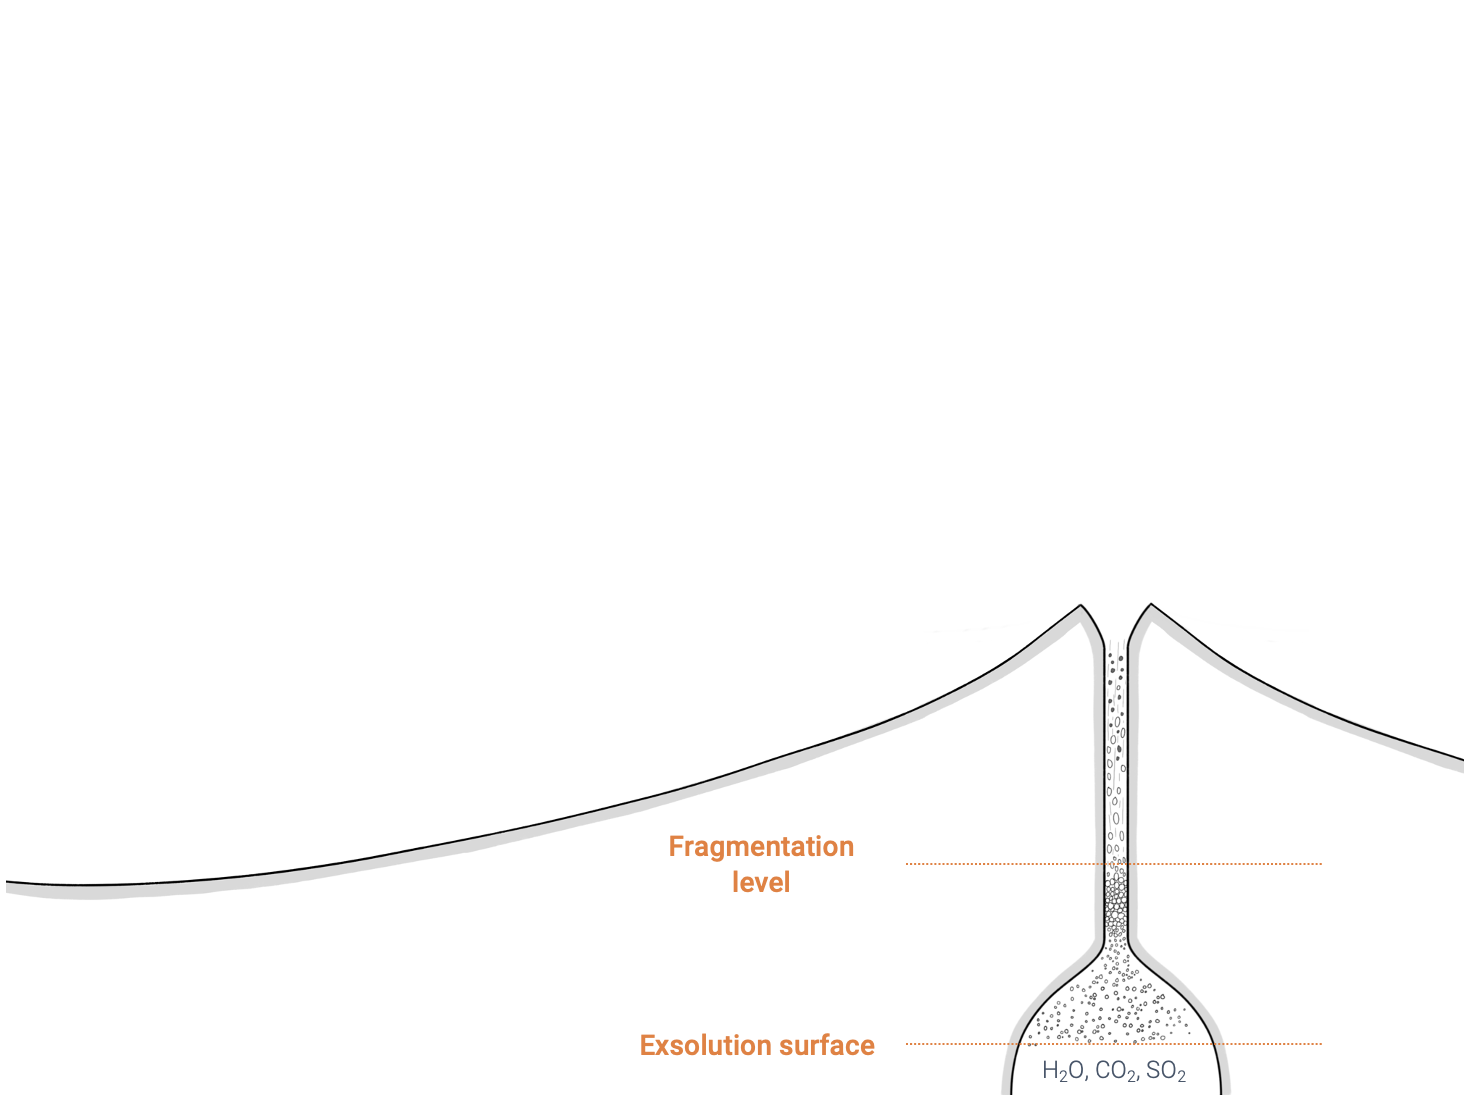
\includegraphics[width=.7\textwidth]{../docs/img/model/m2.png}
    \end{flushright}
  }
  \only<3>{
    \textbf{3. The rise tephra in the atmosphere} $\rightarrow$ the vertical column \\ 
    \begin{flushright}
      \vspace*{-1em}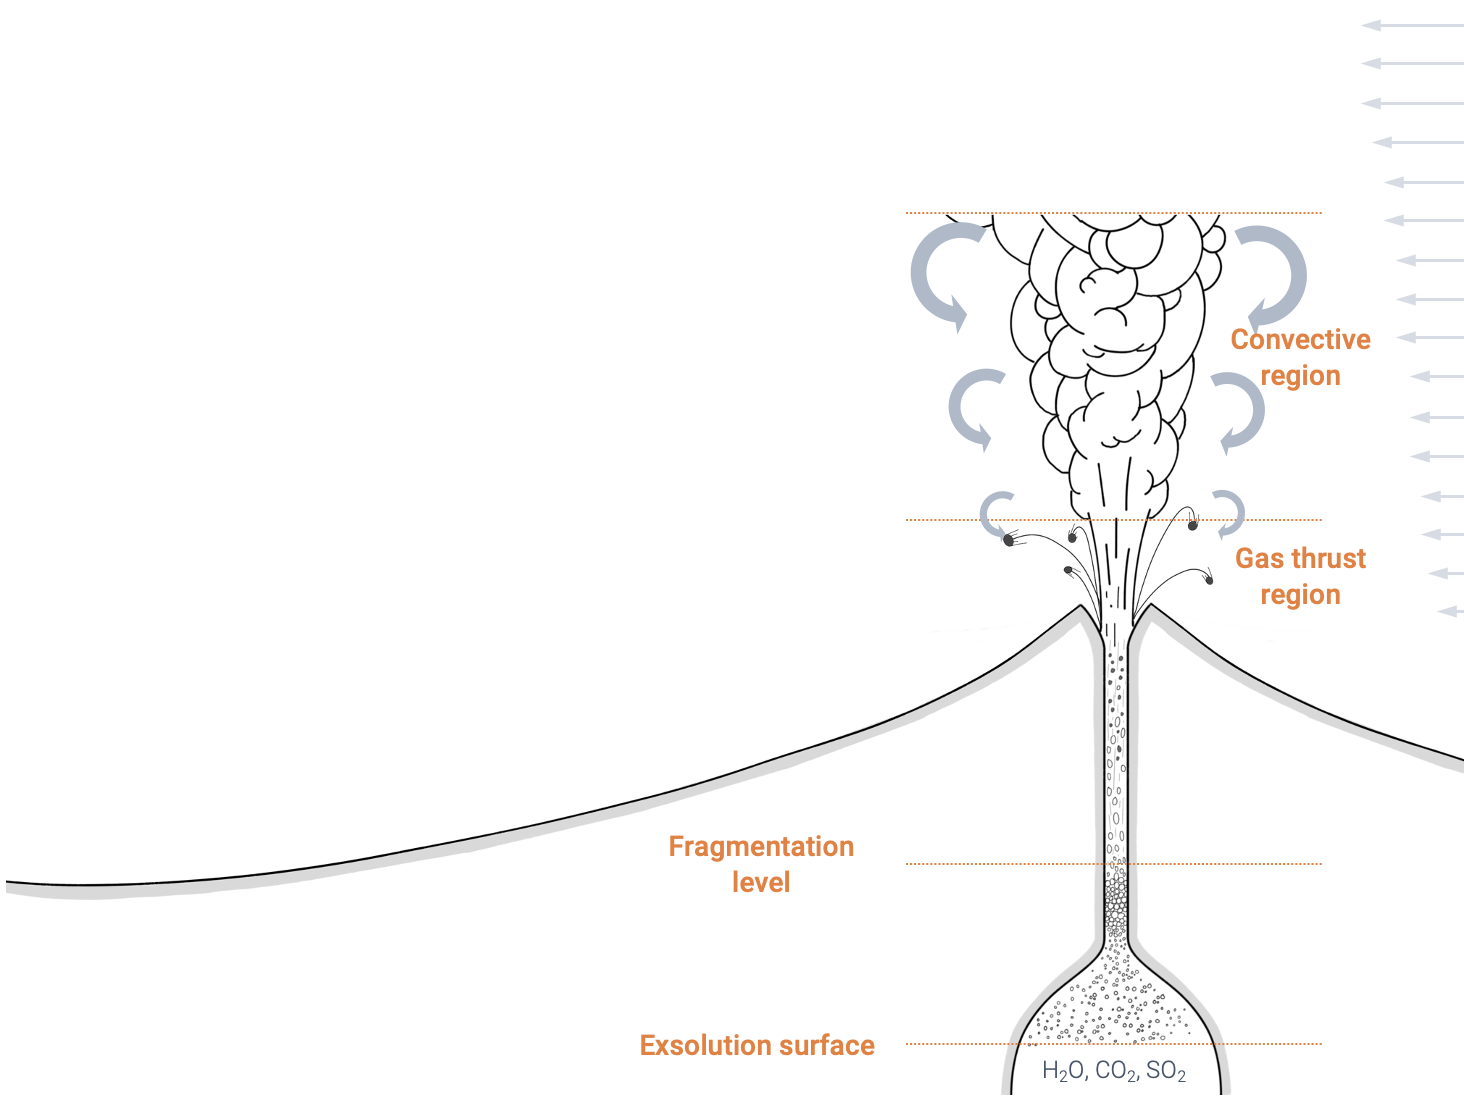
\includegraphics[width=.7\textwidth]{../docs/img/model/m3.png}
    \end{flushright}
  }
  \only<4>{
    \textbf{4. The dispersal by the wind} $\rightarrow$ the "mushroom" cloud \\ 
    \begin{flushright}
      \vspace*{-1em}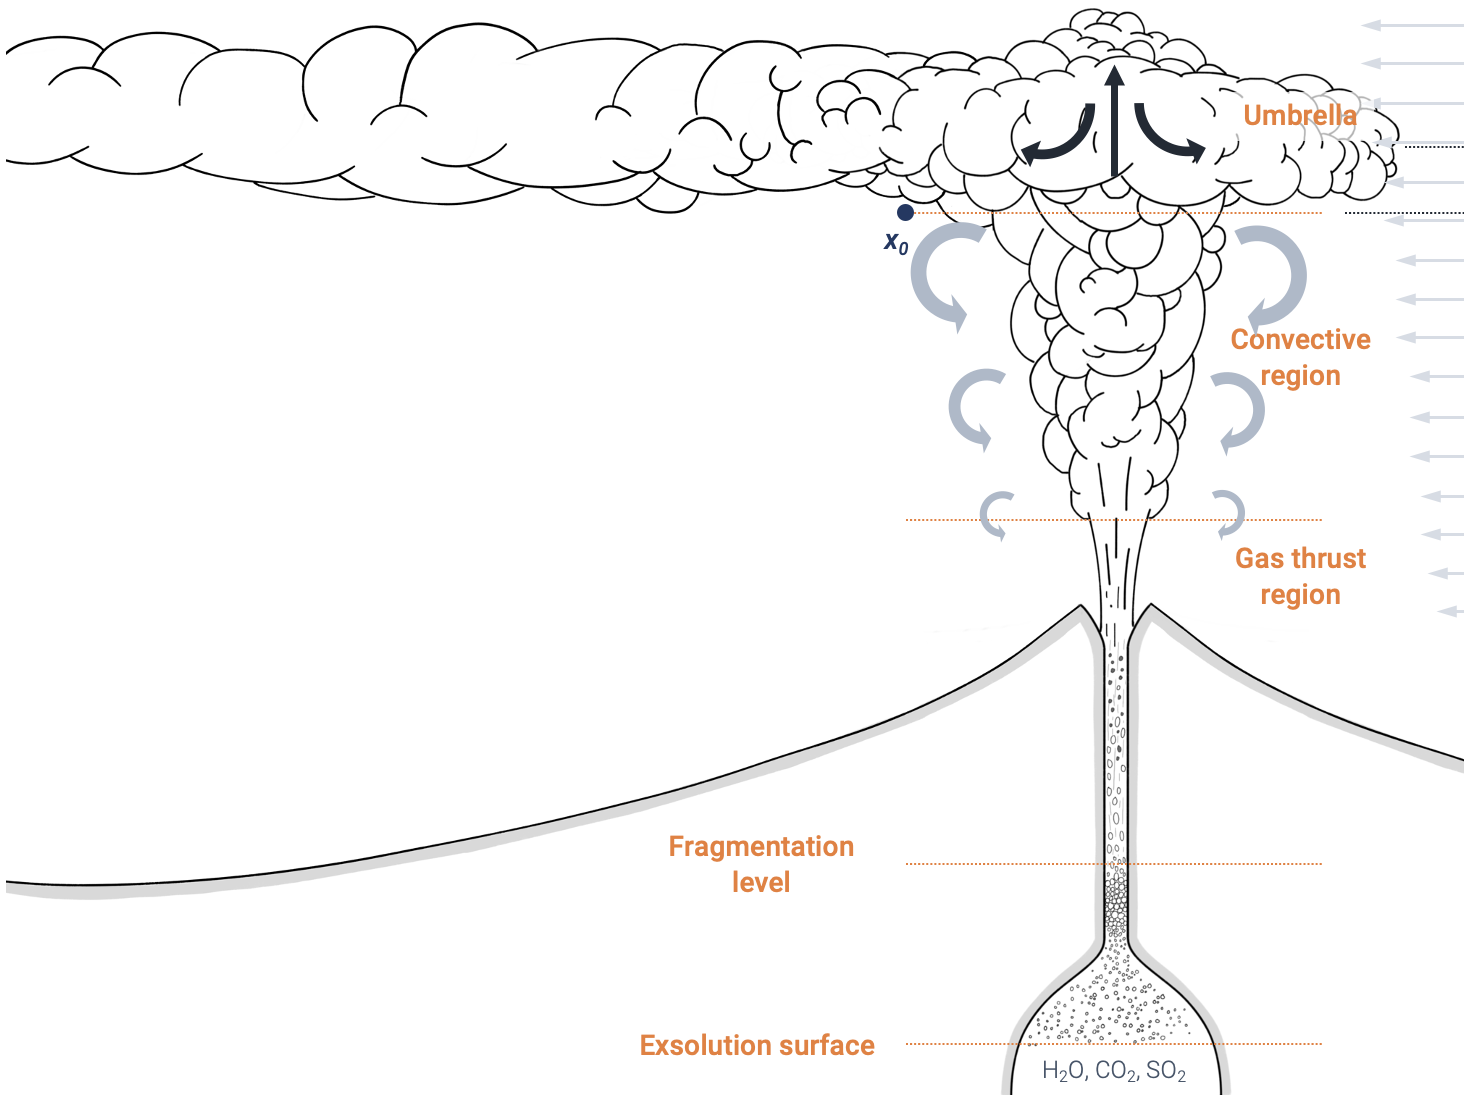
\includegraphics[width=.7\textwidth]{../docs/img/model/m4.png}
    \end{flushright}
  }
  \only<5>{
    \textbf{5. The sedimentation of particles onto the ground } $\rightarrow$ the tephra deposit \\ 
    \begin{flushright}
      \vspace*{-1em}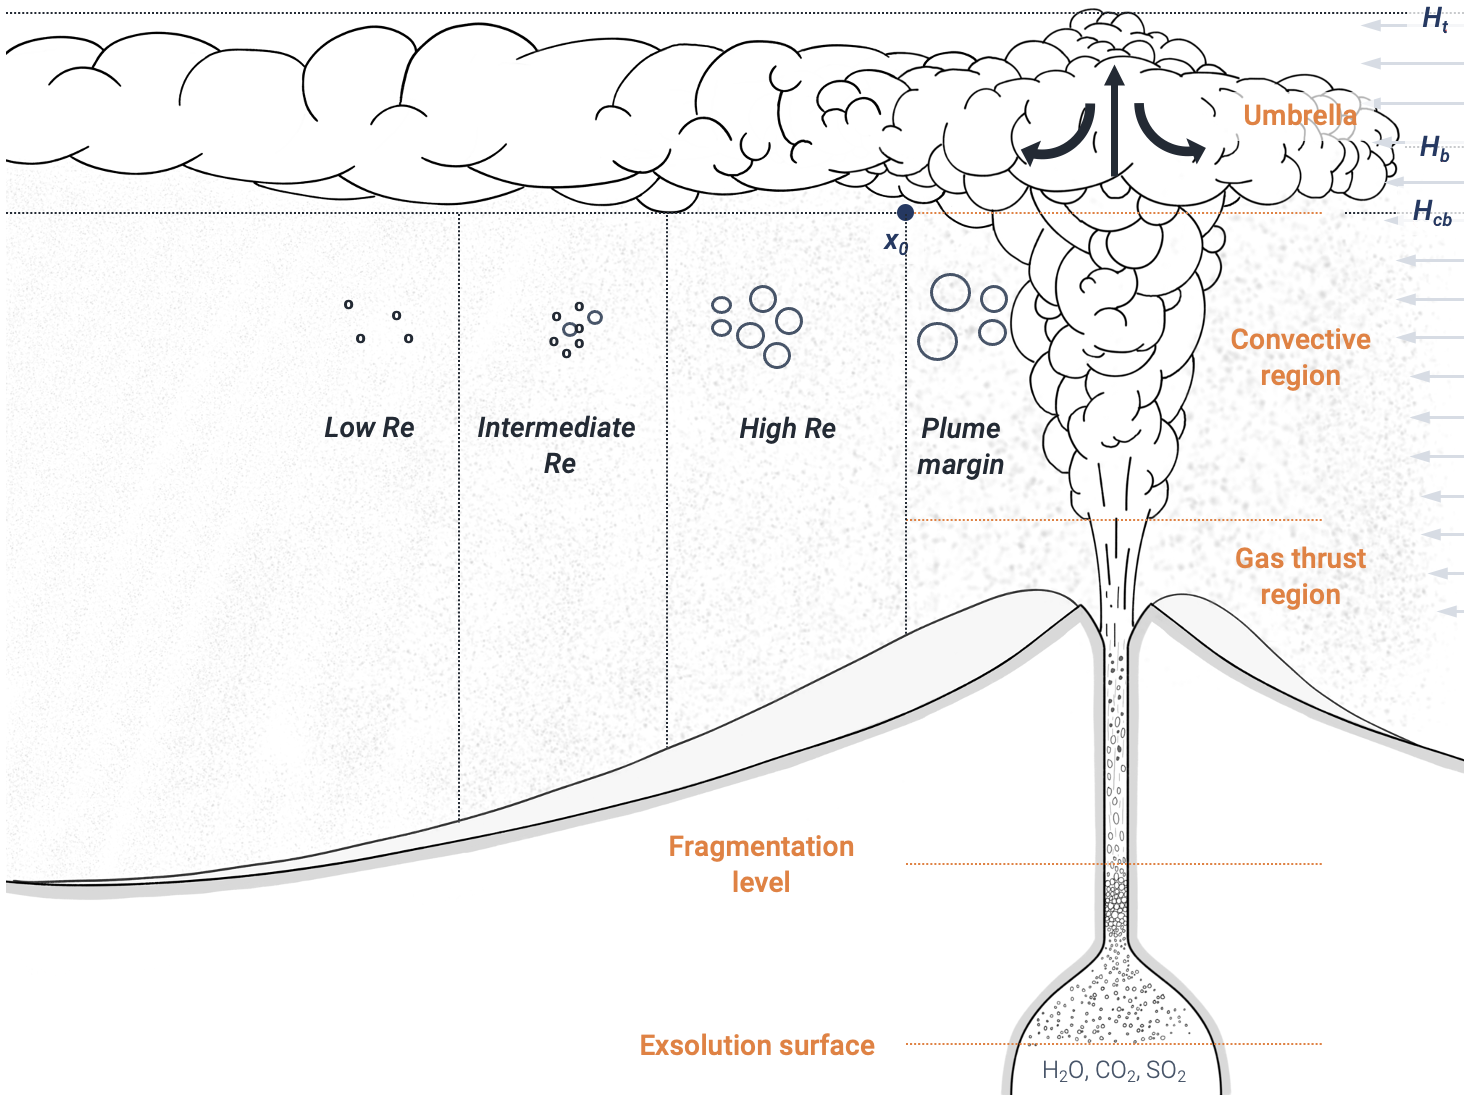
\includegraphics[width=.7\textwidth]{../docs/img/model/m5.png}
    \end{flushright}
  }
\end{frame}



\begin{frame}[t]{Forecasting tephra fallout}

  \begin{columns}[T]
    \begin{column}{0.5\textwidth}	
      \textbf{Tephra2}
      \begin{itemize}
        \item Analytical solution of the advection-diffusion equation
        \item 2D, Eulerian, time-independent
        \item Assumptions $\rightarrow$ fast
      \end{itemize}

      \only<2->{
        \vspace*{1em}
        \textbf{Eruption source parameters}
        \begin{enumerate}
          \item Calculation grid
          \item Wind profiles
          \item Eruption source parameters
          \begin{itemize}
            \item Plume height
            \item Eruption mass
            \item Total grain-size distribution
            \item Plume mass distribution
          \end{itemize}
          
        \end{enumerate}
      }
    \end{column}

    \begin{column}{0.5\textwidth}	
      \only<1-2>{
        \centering 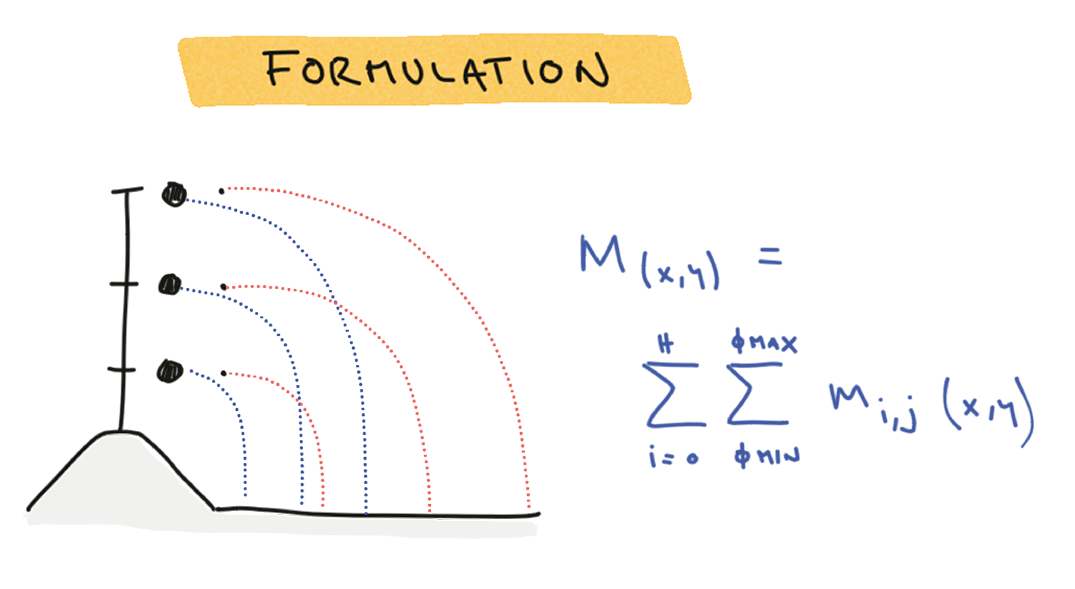
\includegraphics[width=.9\textwidth]{img/tephra2_formulation.png}
        \centering 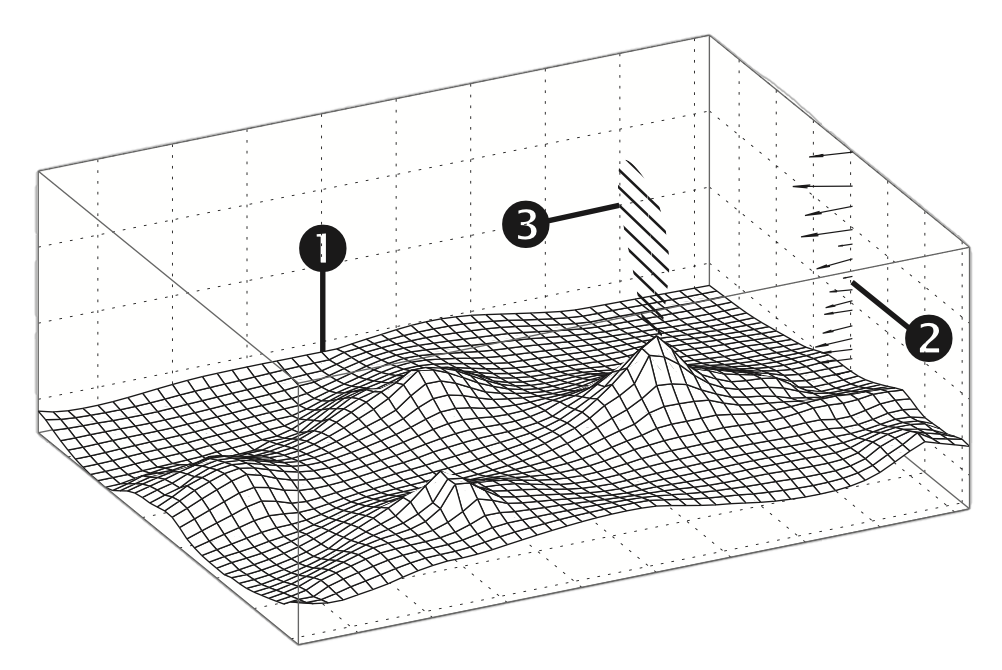
\includegraphics[width=.9\textwidth]{../docs/img/tephra2/tephra2.png}
      }
      \only<3>{
        \centering 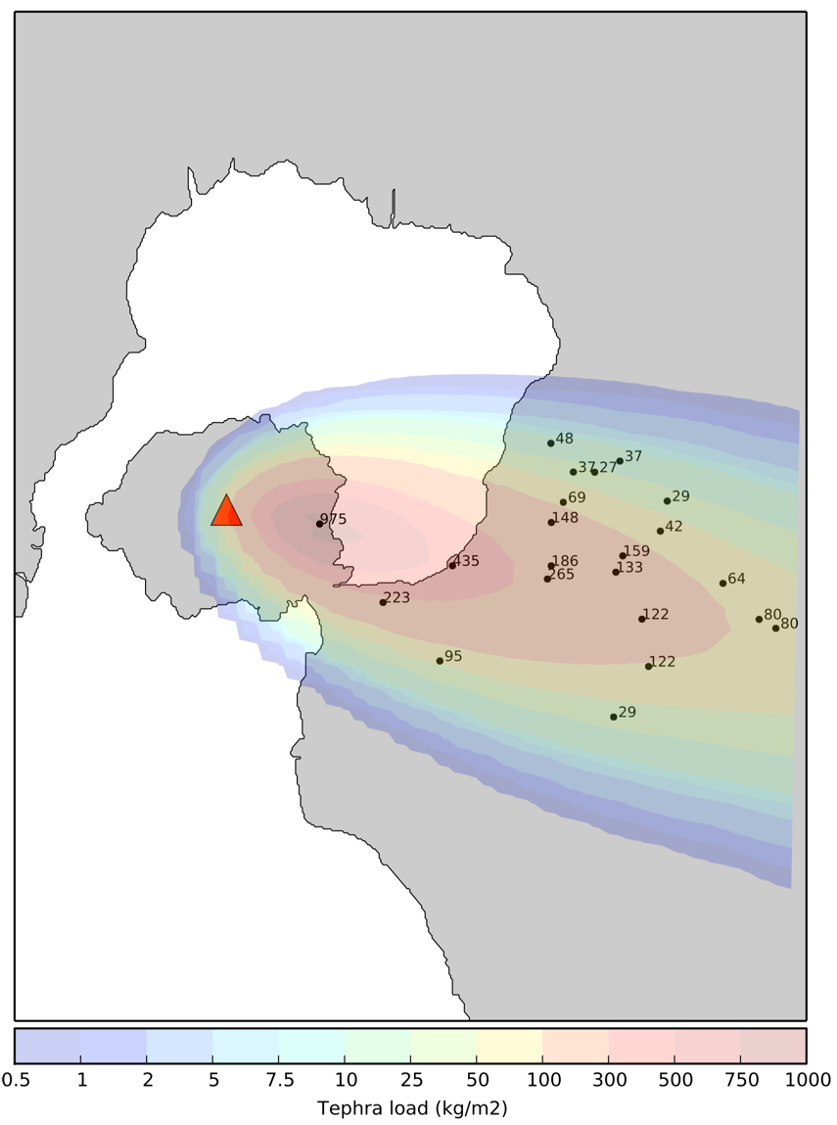
\includegraphics[width=.8\textwidth]{img/tephra2_output.png}
      }
    \end{column}
  \end{columns}

\end{frame}

\begin{frame}[standout]
  Pre--event exposure/impact/risk studies require:\\ \vspace*{1em}
  \alert{$\checkmark$ \textnormal{Ability to \textit{predict} the hazard}}
\end{frame}



\begin{frame}[t]{The missing part}

  \begin{columns}[T]
    \begin{column}{0.5\textwidth}	
      \textbf{What is missing?}
      \vspace*{1em}

      \only<2>{
        \alert{1. The eruptive history...}\\ \vspace*{1em}
        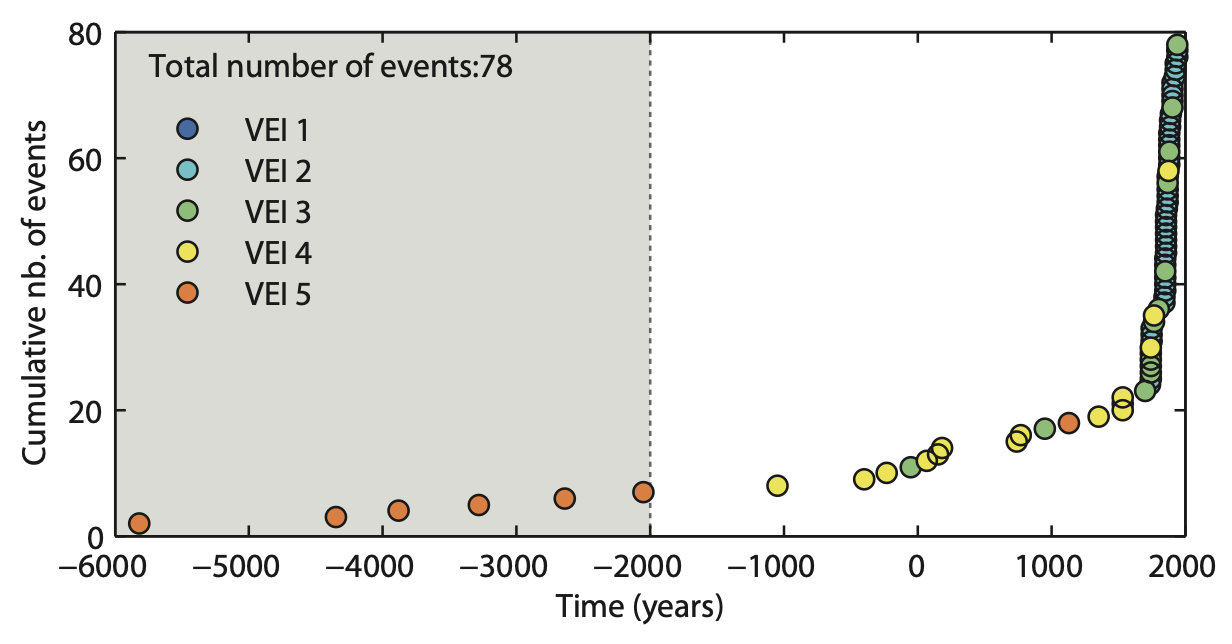
\includegraphics[width=1\textwidth]{../docs/img/cotopaxi/gvp.png}
      }
      \only<3>{
        \alert{2. The atmpospheric variability...}\\ \vspace*{1em}
        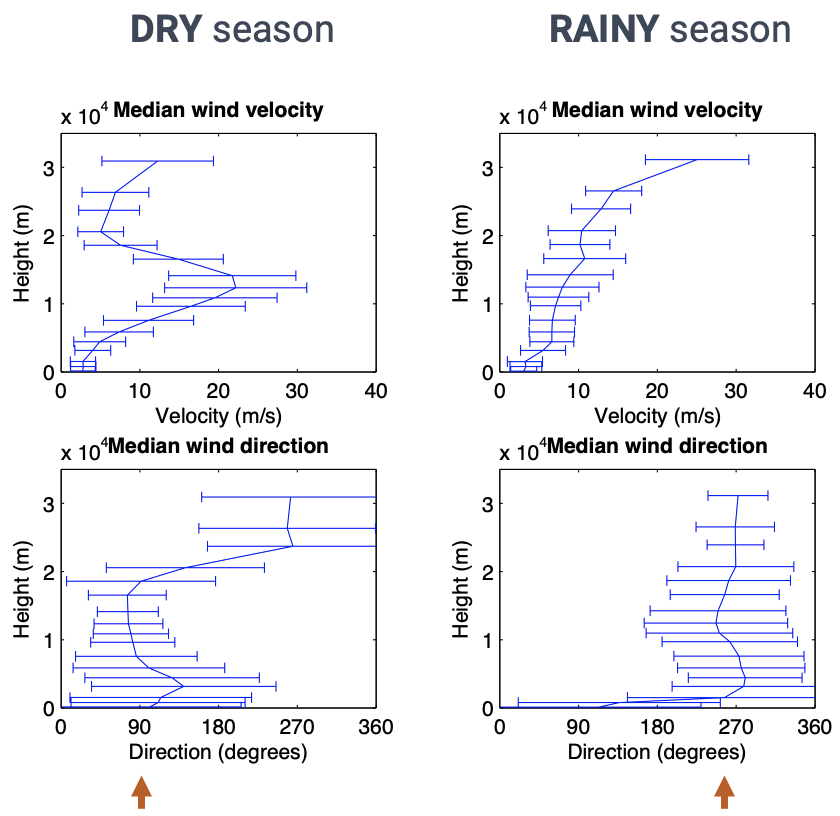
\includegraphics[width=.9\textwidth]{../docs/img/cotopaxi/wind.png}
      }
    \end{column}

    \begin{column}{0.5\textwidth}	
      \centering 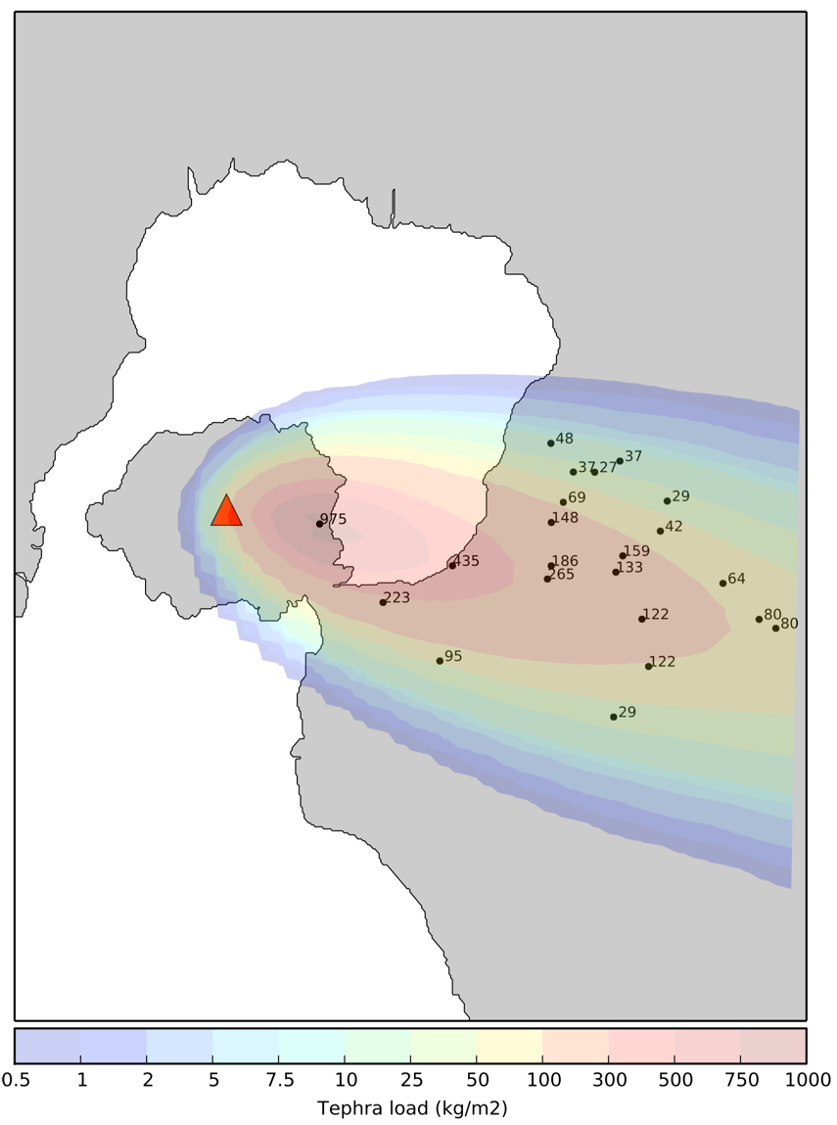
\includegraphics[width=.8\textwidth]{img/tephra2_output.png}
    \end{column}
  \end{columns}

\end{frame}

\begin{frame}[standout]
  Pre--event exposure/impact/risk studies require:\\ \vspace*{1em}
  \alert{$\checkmark$ \textnormal{Ability to \textit{predict} the hazard}}\\
  $\rightarrow$ \textnormal{Ability to describe the \textit{variability} of eruptive conditions}
\end{frame}


\section{\alert{Tephra fallout part II} \\ Probabilistic hazard modeling}

\begin{frame}[t]{Deterministic to probabilistic modeling}

  \only<1-2>{
  \begin{columns}[T]
    \begin{column}{0.5\textwidth}	
      \alert<1>{\textbf{Lava flows:}}
      \begin{itemize}
        \item \textbf{Input}: Uncertainty on \alert{DEM} + \alert{vent location}
        \item \textbf{Hazard metrics}: Boolean yes/no inundation
        \item \textbf{Output}: Probability of flow inundation
      \end{itemize}

      \only<2>{
        \vspace*{1em}
        \alert<2>{\textbf{Tephra fallout:}}
        \begin{itemize}
          \item \textbf{Input}: Uncertainty on \alert{ESP} + \alert{wind}
          \item \textbf{Hazard metrics}: Tephra load ($kg/m^2$)
          \item \textbf{Output}: Probability to exceed tephra load
        \end{itemize}
      }

    \end{column}

    \begin{column}{0.5\textwidth}	
      \only<1>{\centering 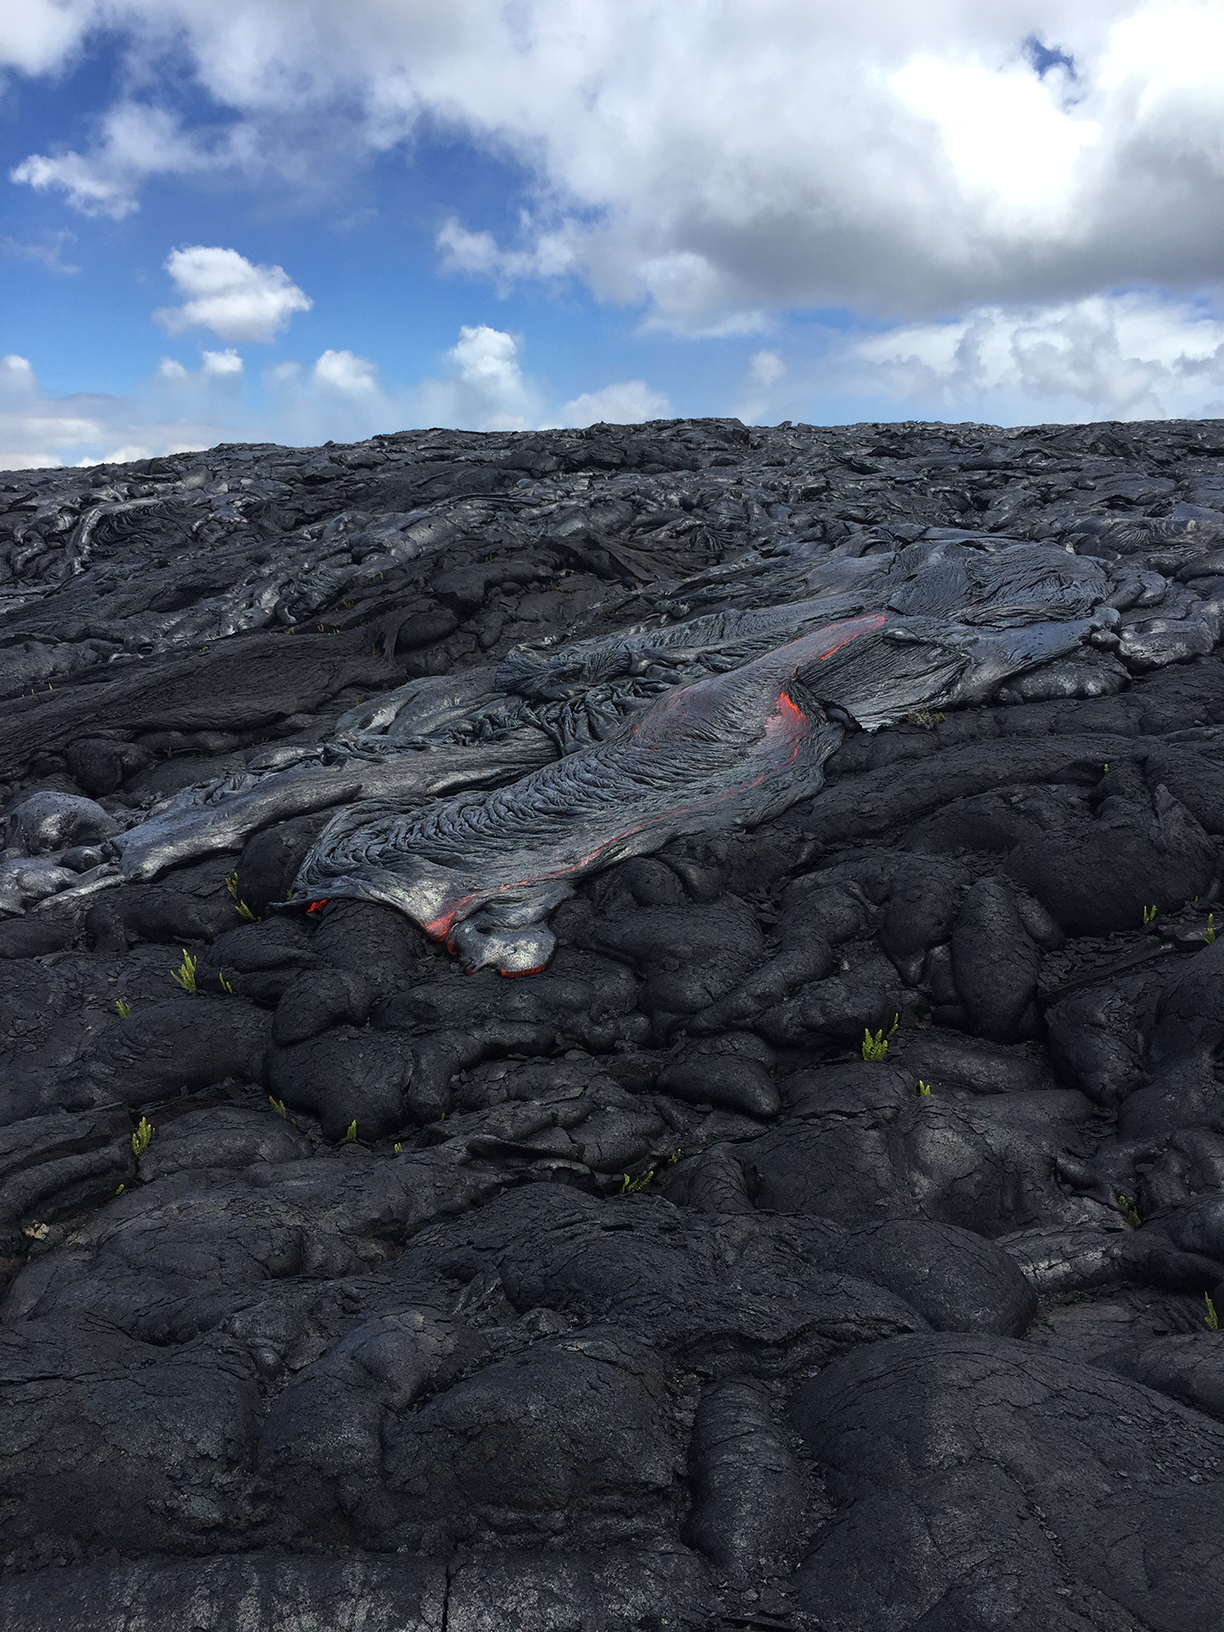
\includegraphics[width=.8\textwidth]{../docs/img/61g/toes.png}}
      \only<2>{\centering 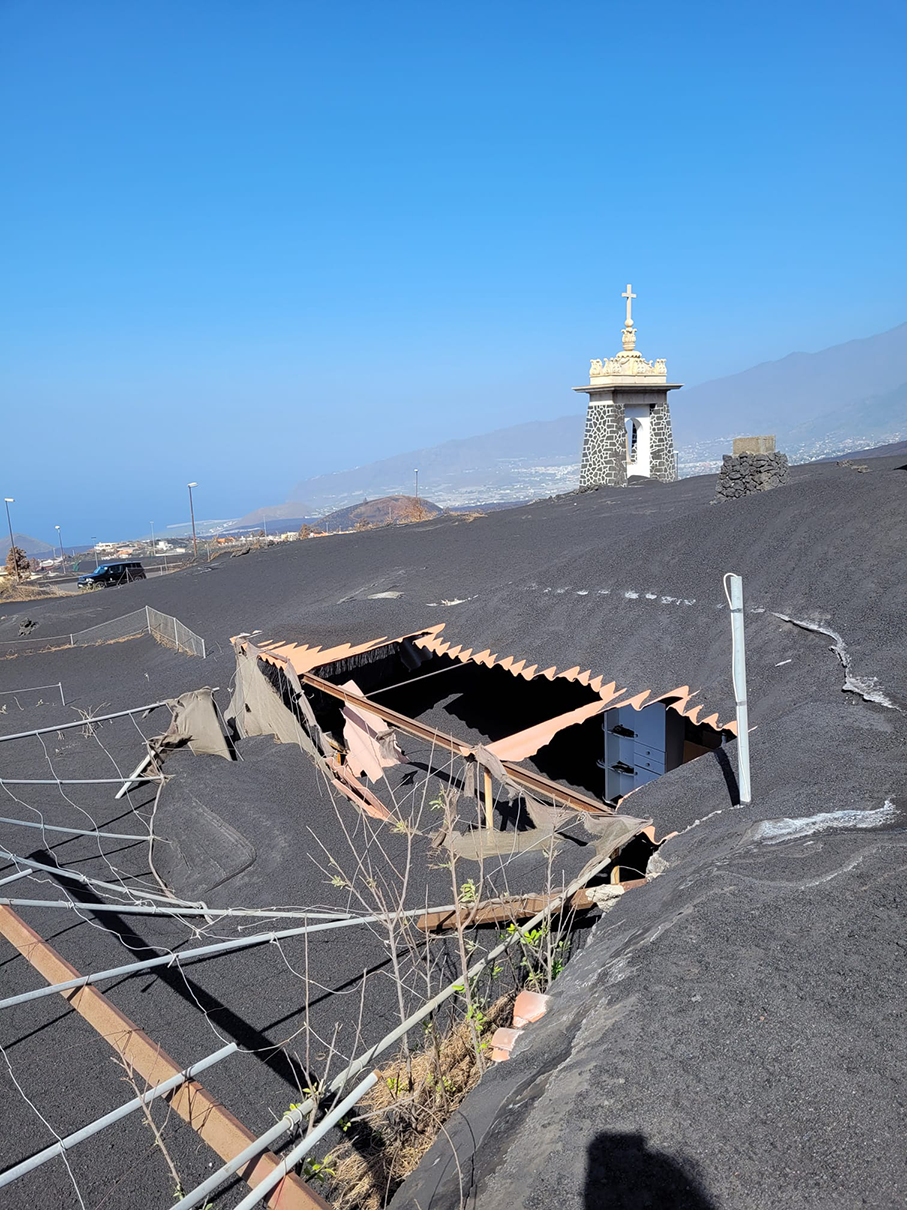
\includegraphics[width=.8\textwidth]{img/tephra_thickness.png}}
    \end{column}
  \end{columns}
  }
  \only<3>{\vspace*{3em}\centering 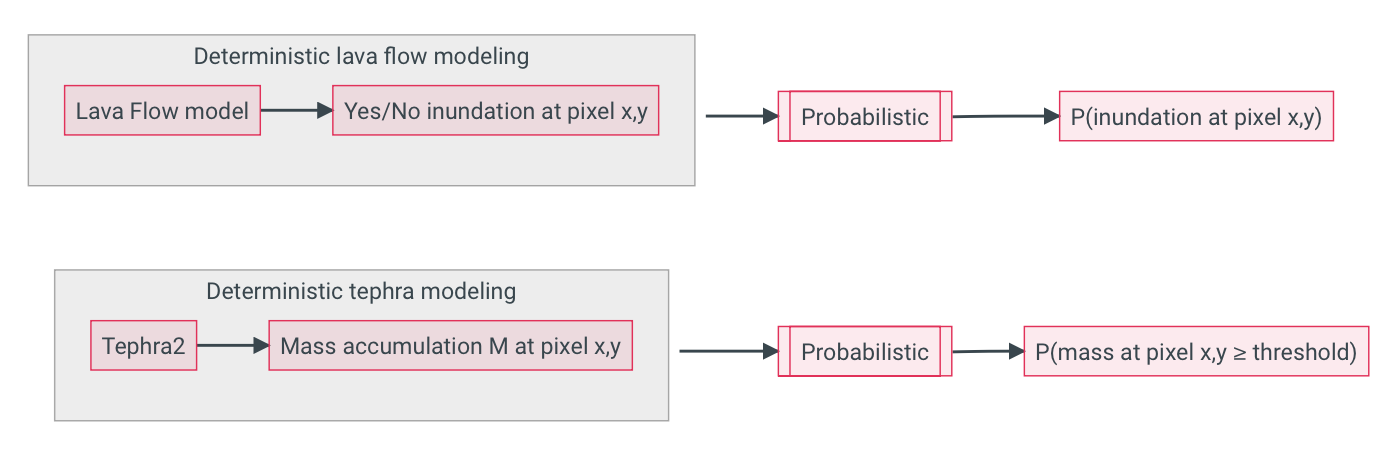
\includegraphics[width=1\textwidth]{img/prob_lava-vs-tephra.png}}

\end{frame}



\begin{frame}[t]{Probabilistic eruption scenarios}

  \centering \textbf{ESP for Tephra2:} \alert{Plume height}, \alert{erupted mass/volume}, \alert{grain-size distribution}\\
  \flushleft

  \vspace*{1em}
  \only<1>{
  \textbf{Workflow:}
  \begin{itemize}
    \item Identify the relevant \textbf{Eruption Source Parameters} (ESP) for model/problem 
    \item For each ESP, define:
    \begin{itemize}
      \item \alert{Range}
      \item \alert{Distribution}
    \end{itemize}
  \end{itemize}
  \centering 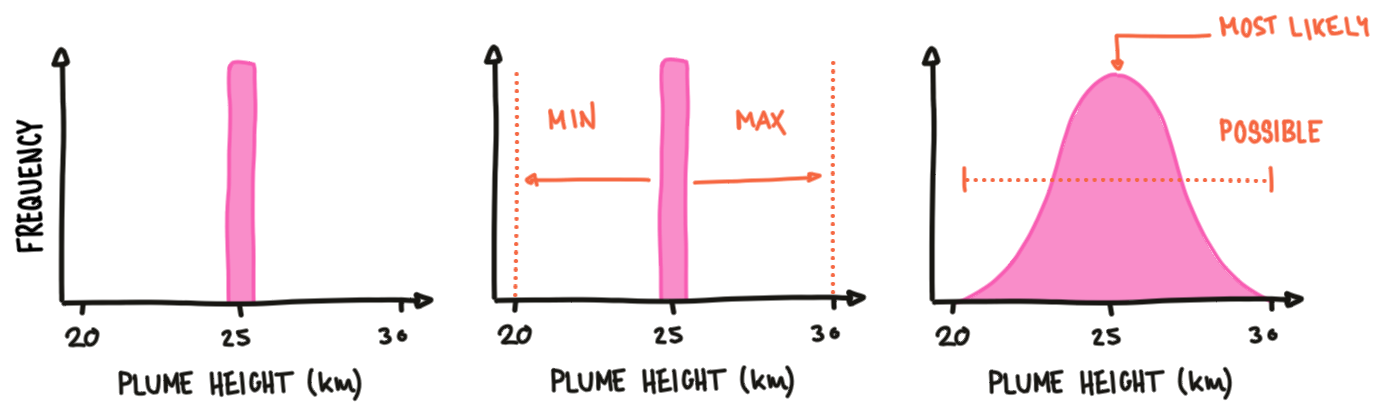
\includegraphics[width=.8\textwidth]{../docs/img/ESP/ESP-scenarios.png}
  }
  
  \only<2>{
    \textbf{Definition:} Eruption scenarios can be developed around:
    \begin{itemize}
      \item Reference eruption
      \item VEI
      \item Intensity
      \item Eruptive style
      \item ...
    \end{itemize}

    \vspace*{1em}
    \centering $\rightarrow$ \alert{The \textbf{purpose} of the study influences \textbf{how} a scenario is developed!}

  }

\end{frame}


\begin{frame}{A note about uncertainties}

  \only<1>{

  \centering \textbf{Uncertainties:}\\
    \vspace*{1em}
    $\rightarrow$ \alert{Epistemic uncertainties}: derives from the \alert{lack of knowledge} regarding a phenomena. In theory, we could reduce it with more \alert{knowledge}.\\ \vspace*{1em}
    $\rightarrow$ \alert{Aleatoric uncertainties}: associated with the inherent \alert{randomness} of natural processes. Nothing much we can do about it, really!
  }
  
  \only<2>{
    \begin{columns}[T]
      \begin{column}{0.45\textwidth}	
        \textbf{ESP distributions}:\vspace*{1em}
        \begin{itemize}
          \item Account for both \alert{epistemic} and \alert{aleatory} uncertainties
          \item Reflect our \alert{knowledge} of the system
          \item Based on:
          \begin{itemize}
            \item[$\rightarrow$] Ideally, \alert{field studies} 
            \item[$\rightarrow$] \alert{Literature} reviews 
            \item[$\rightarrow$] \alert{Analogue} volcanoes/eruptions 
            \item[$\rightarrow$] Eruption \alert{databases}
          \end{itemize}
        \end{itemize}
        
      \end{column}
      
      \begin{column}{0.55\textwidth}	
        
        \centering 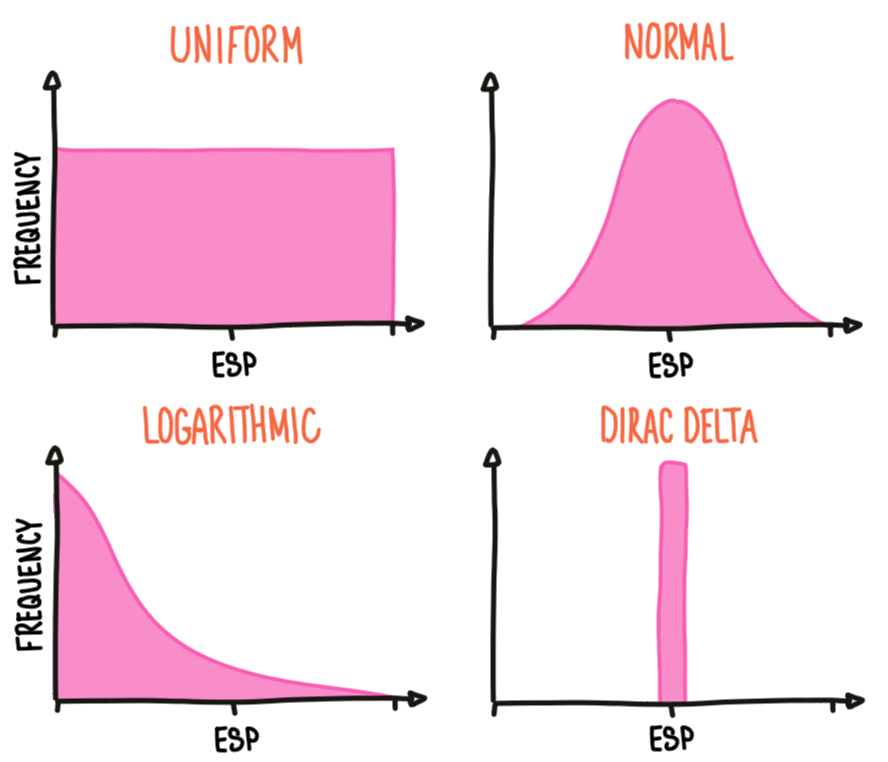
\includegraphics[width=1\textwidth]{../docs/img/ESP/ESP-distributions.png}
    \end{column}
  \end{columns}
  }
\end{frame}



\begin{frame}{Probabilistic modeling}

  \only<1>{
  We are studying the famous \textbf{Mt. Bonadonna} volcano --- a majestic but at time deadly volcano. Based on our knowledge (and fear) of it, we defined the following \alert{eruption scenario}: 

  \begin{itemize}
    \item \textbf{VEI 4} $\rightarrow 10^{11}-10^{12}$ kg of tephra, Gaussian distribution
    \item \textbf{Plume height:} 20--30 km asl, Gaussian distribution
    \item \textbf{Wind conditions:} 20 years from \alert{Reanalysis} databases
  \end{itemize}
  \vspace*{1em}
  \centering 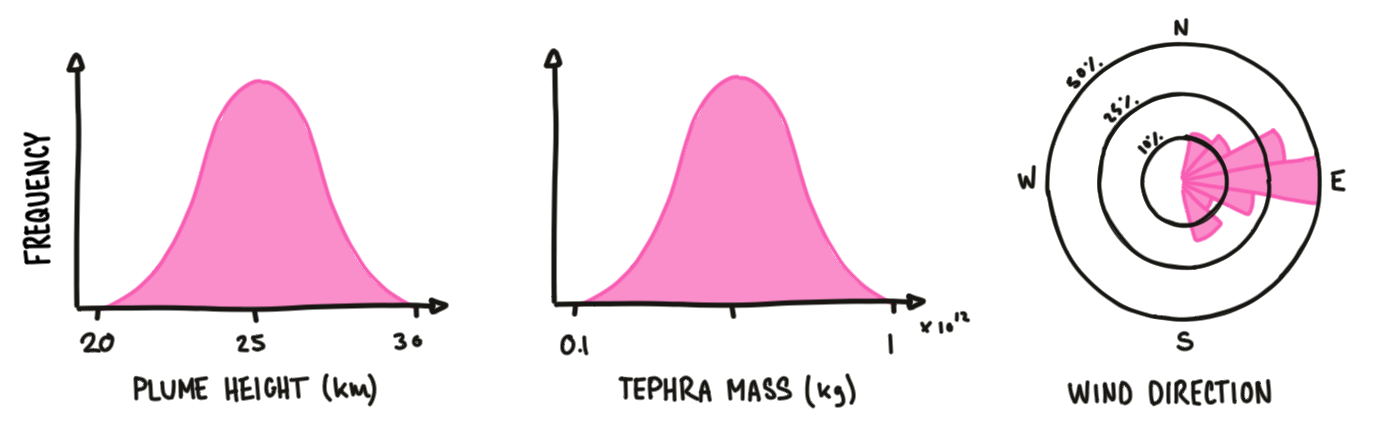
\includegraphics[width=.9\textwidth]{../docs/img/scenario/esp_scenario_0.png}
  }  
  
  \only<2>{
    \centering 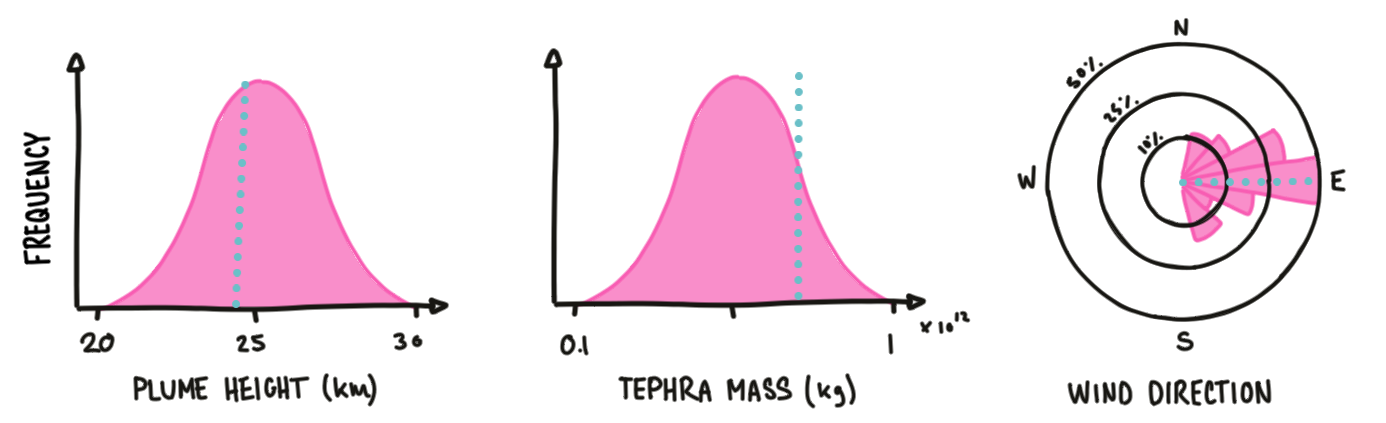
\includegraphics[width=.85\textwidth]{../docs/img/scenario/esp_scenario_1.png}\\
    \centering 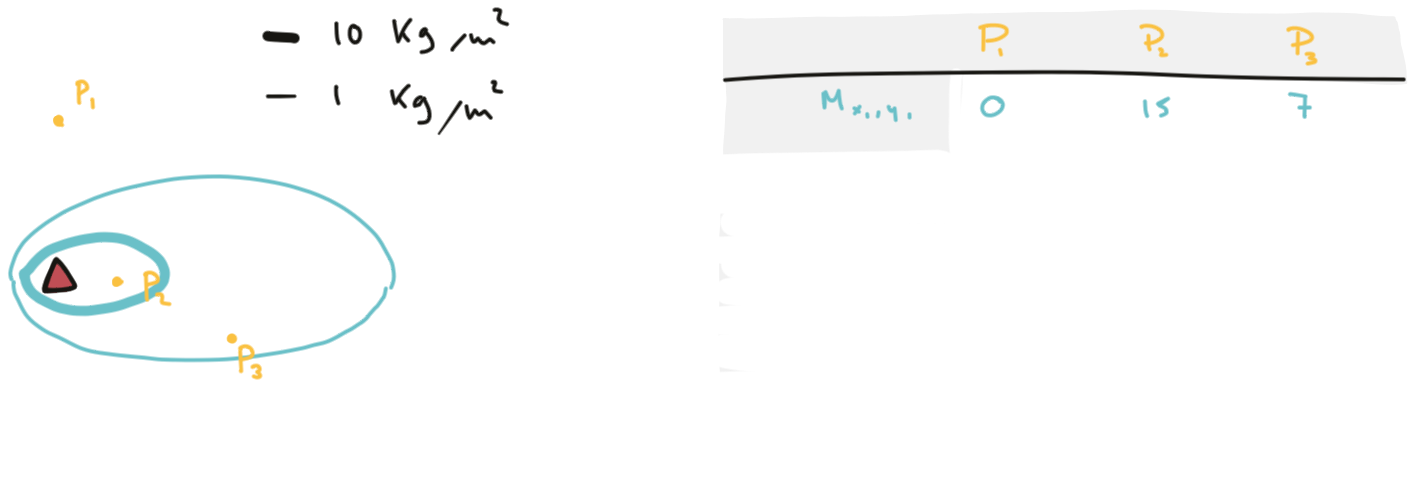
\includegraphics[width=.85\textwidth]{../docs/img/scenario/tephra_prob1.png}
  }
  \only<3>{
    \centering 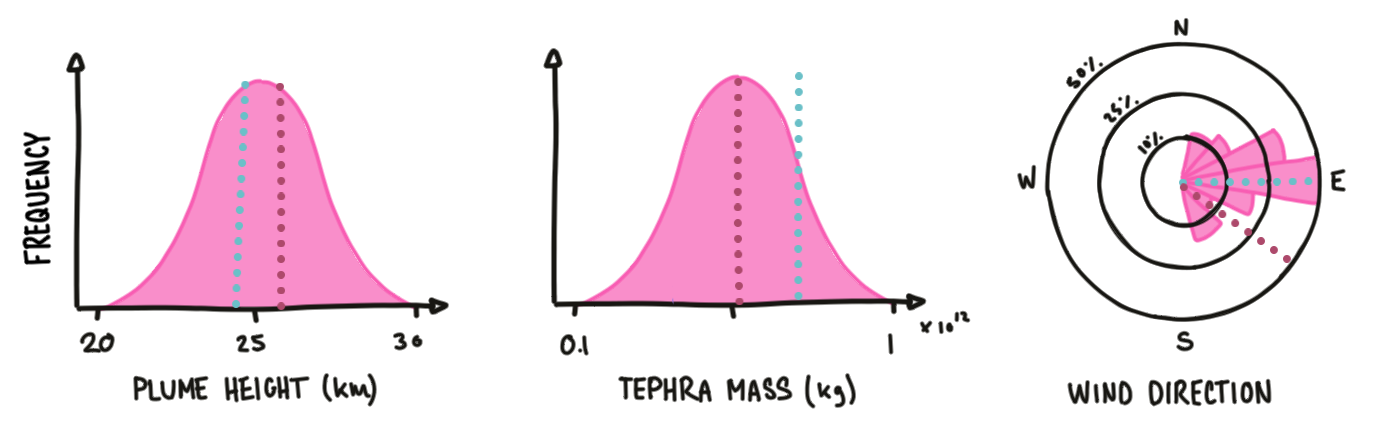
\includegraphics[width=.85\textwidth]{../docs/img/scenario/esp_scenario_2.png}\\
    \centering 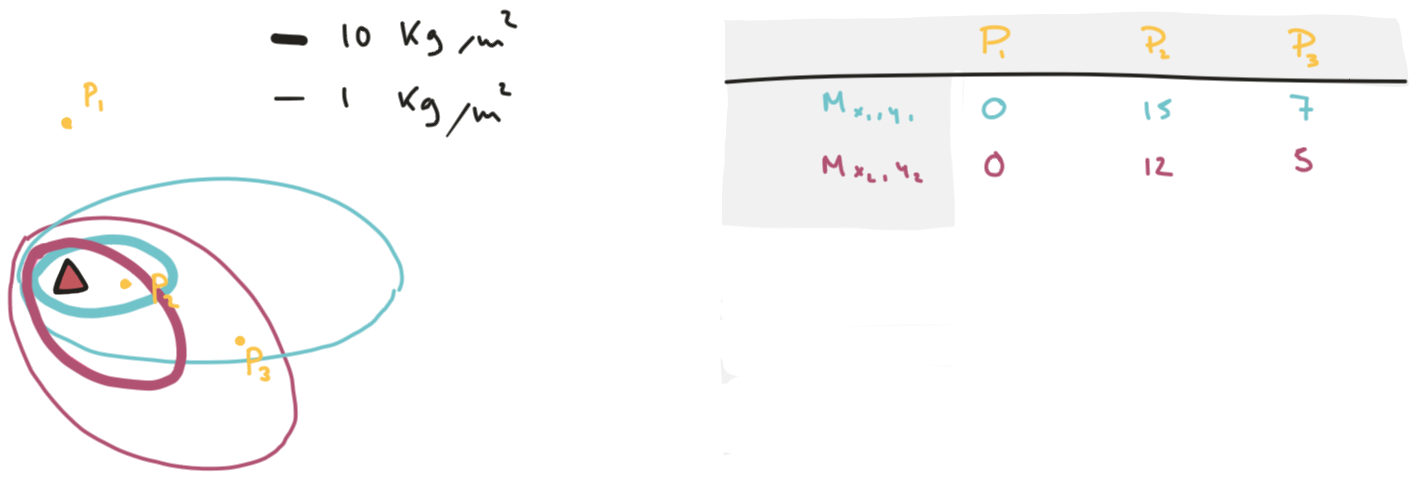
\includegraphics[width=.85\textwidth]{../docs/img/scenario/tephra_prob2.png}
  }
  \only<4>{
    \centering 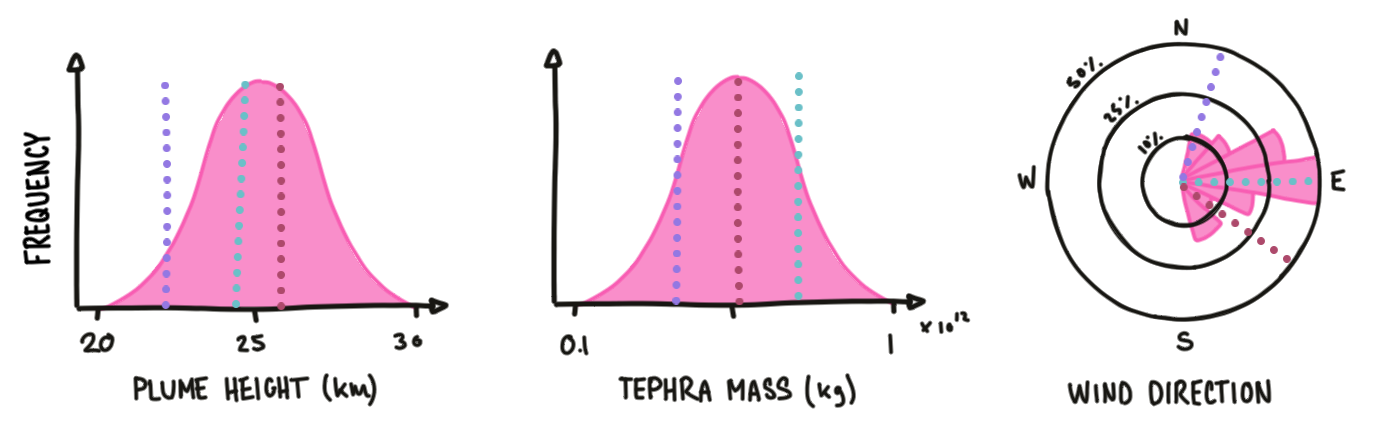
\includegraphics[width=.85\textwidth]{../docs/img/scenario/esp_scenario_3.png}\\
    \centering 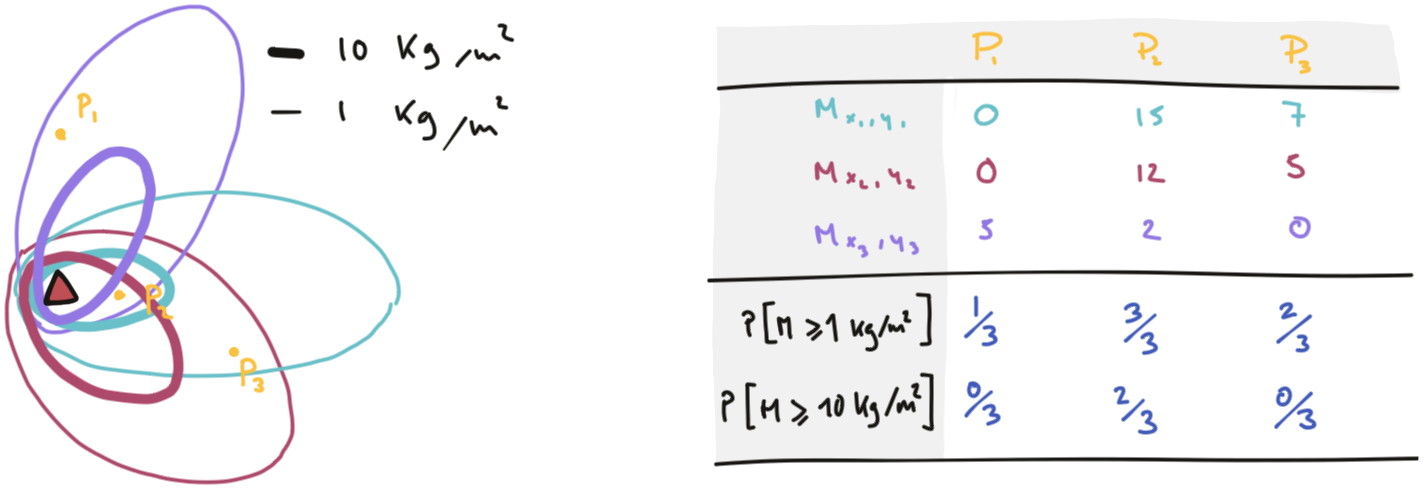
\includegraphics[width=.85\textwidth]{../docs/img/scenario/tephra_prob3.png}
  }

\end{frame}

\begin{frame}[standout]
  Pre--event exposure/impact/risk studies require:\\ \vspace*{1em}
  \alert{$\checkmark$ \textnormal{Ability to \textit{predict} the hazard}}\\
  \alert{$\checkmark$ \textnormal{Ability to describe the \textit{variability} of eruptive conditions}}
\end{frame}

\begin{frame}[standout]
  How to display hazard outputs?
\end{frame}

\begin{frame}{Probabilistic hazard visualisation}
  \begin{itemize}
    \item For \textbf{lava flows}, there were 3 quantities to represent: \alert{easting} (longitude), \alert{northing} (latitude) and \alert{probability} \vspace*{1em}
    \item For \textbf{tephra fallout}, we have another quantity to represent: \alert{tephra accumulation}\vspace*{1em}
    \item There are \textbf{4} quantities $\rightarrow$ \alert{one too many to represent on a single map}!
  \end{itemize}
\end{frame}

\begin{frame}{Method 1: Probability maps}
  \only<1>{
    \begin{columns}[T]
      \begin{column}{0.65\textwidth}	
        \textbf{Probabilistic hazard maps}:\vspace*{1em}
        \begin{itemize}
          \item \alert{Fixed threshold} of tephra accumulation \vspace*{1em}
          \item Other quantities are expressed \alert{continuously} \vspace*{1em}
          \item Display the \alert{spatial distribution} of exceedence probabilities of a single threshold of tephra accumulation  \vspace*{1em}
          \item There are \alert{as many maps} as accumulation thresholds \vspace*{1em}
        \end{itemize}
        
      \end{column}
      
      \begin{column}{0.35\textwidth}	
        \centering 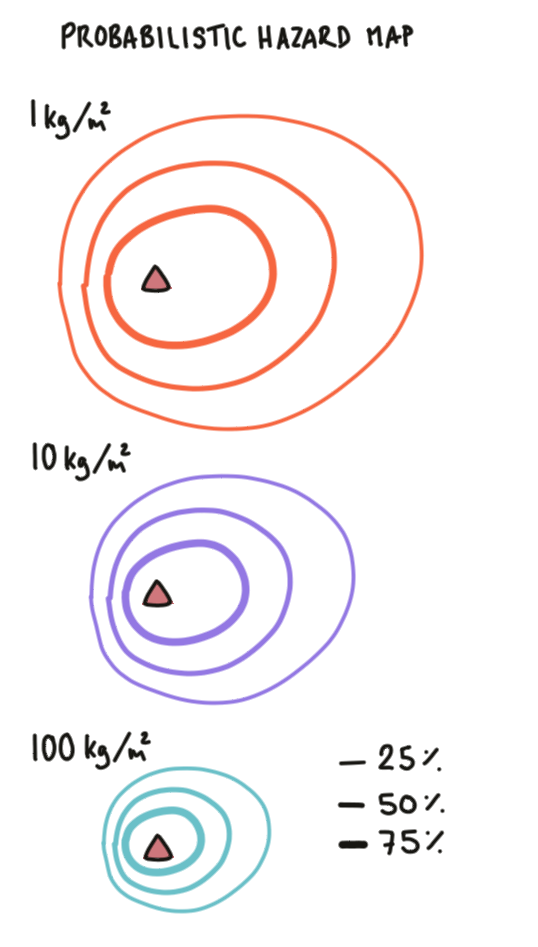
\includegraphics[width=.9\textwidth]{img/prob_map.png}
      \end{column}
    \end{columns}
  }
  \only<2>{
    \centering 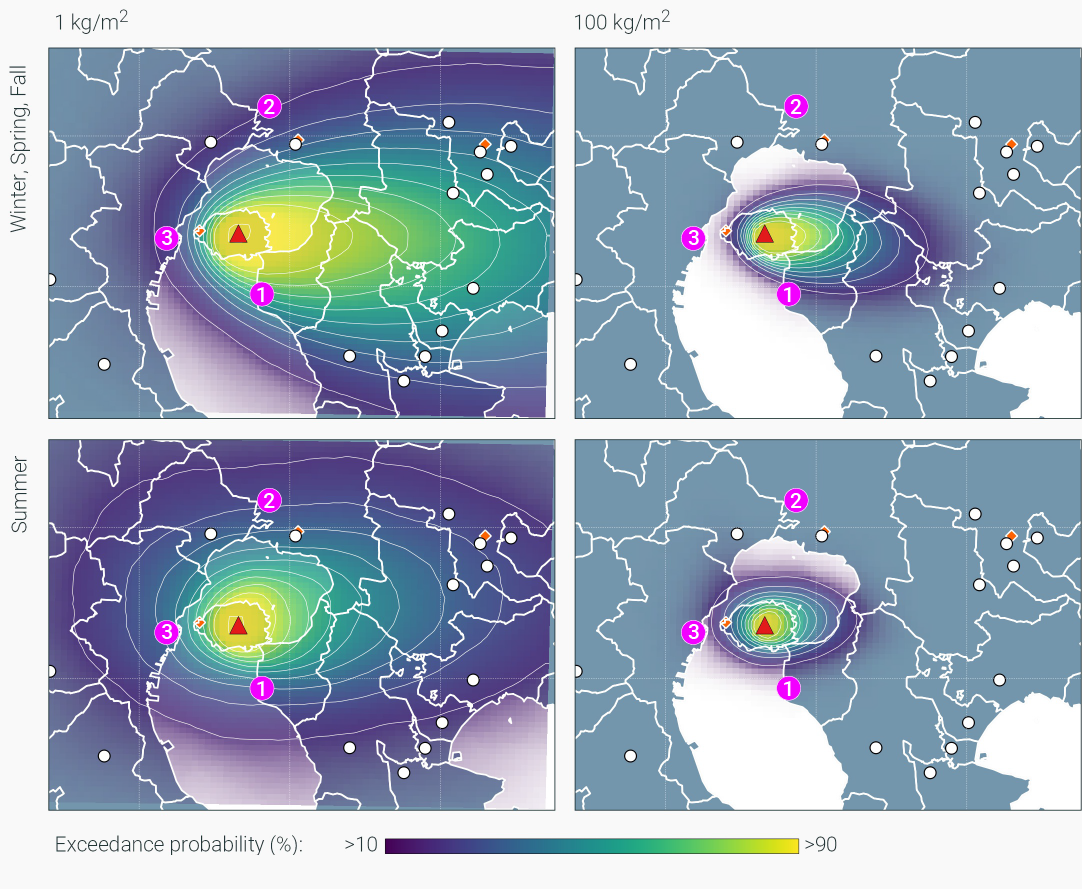
\includegraphics[width=.7\textwidth]{../docs/img/sakurajima/prob.png}
    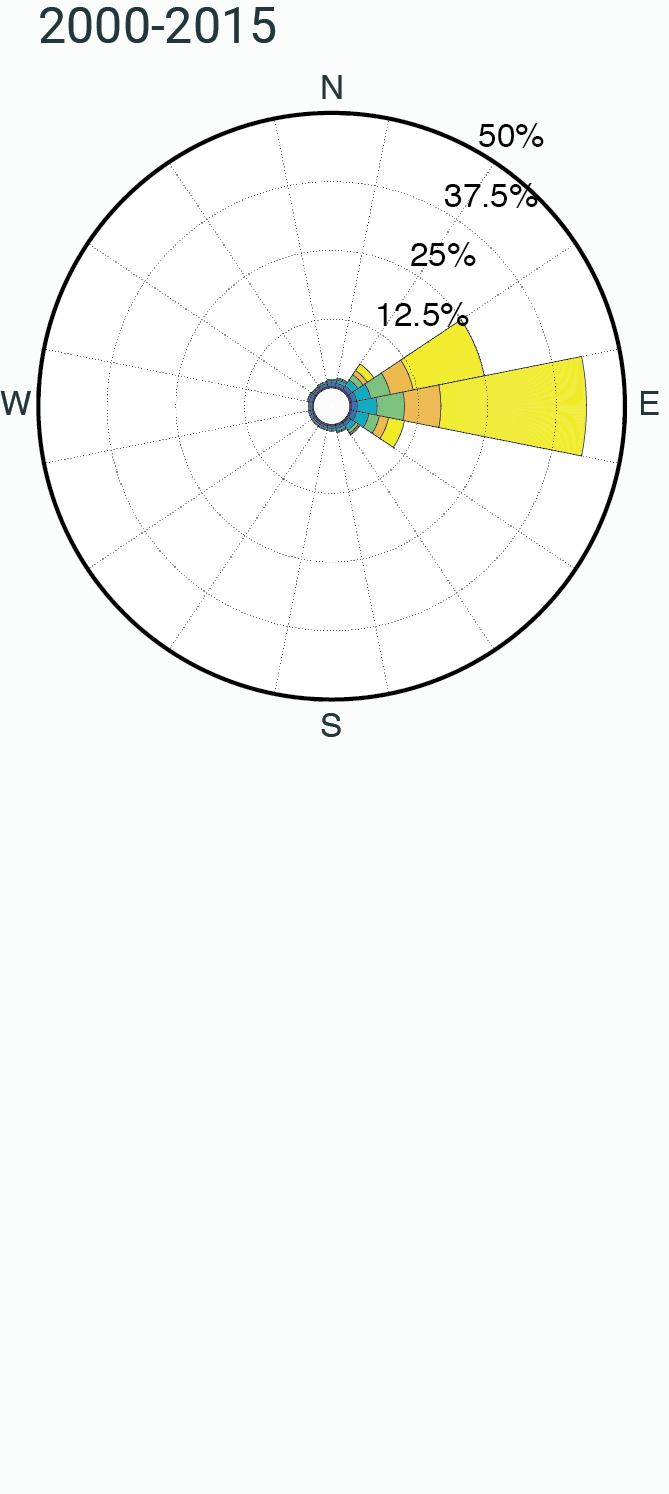
\includegraphics[width=.25\textwidth]{img/wind_all.png}
  }
\end{frame}


\begin{frame}{Method 2: Probabilistic isomass maps}
  \only<1>{
    \begin{columns}[T]
      \begin{column}{0.65\textwidth}	
        \textbf{Probabilistic isomass maps}:\vspace*{1em}
        \begin{itemize}
          \item \alert{Fixed threshold} of exceedence probability \vspace*{1em}
          \item Other quantities are expressed \alert{continuously} \vspace*{1em}
          \item Display the \alert{spatial distribution} of exceedence probabilities for a single exceedence probability value \vspace*{1em}
          \item There are \alert{as many maps} as probability values \vspace*{1em}
        \end{itemize}

      \end{column}
      
      \begin{column}{0.35\textwidth}	
        \centering 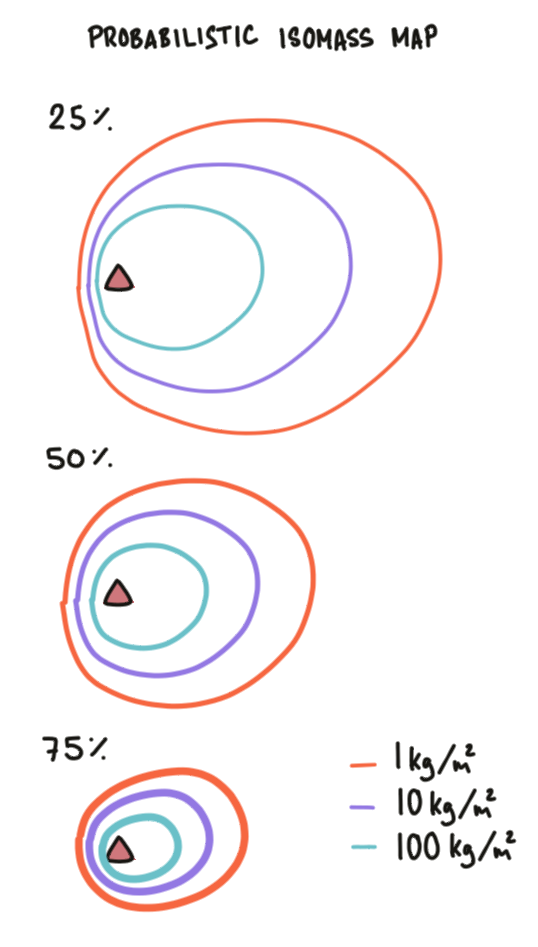
\includegraphics[width=.9\textwidth]{img/isomass_map.png}
      \end{column}
    \end{columns}
  }
  \only<2>{
    \centering 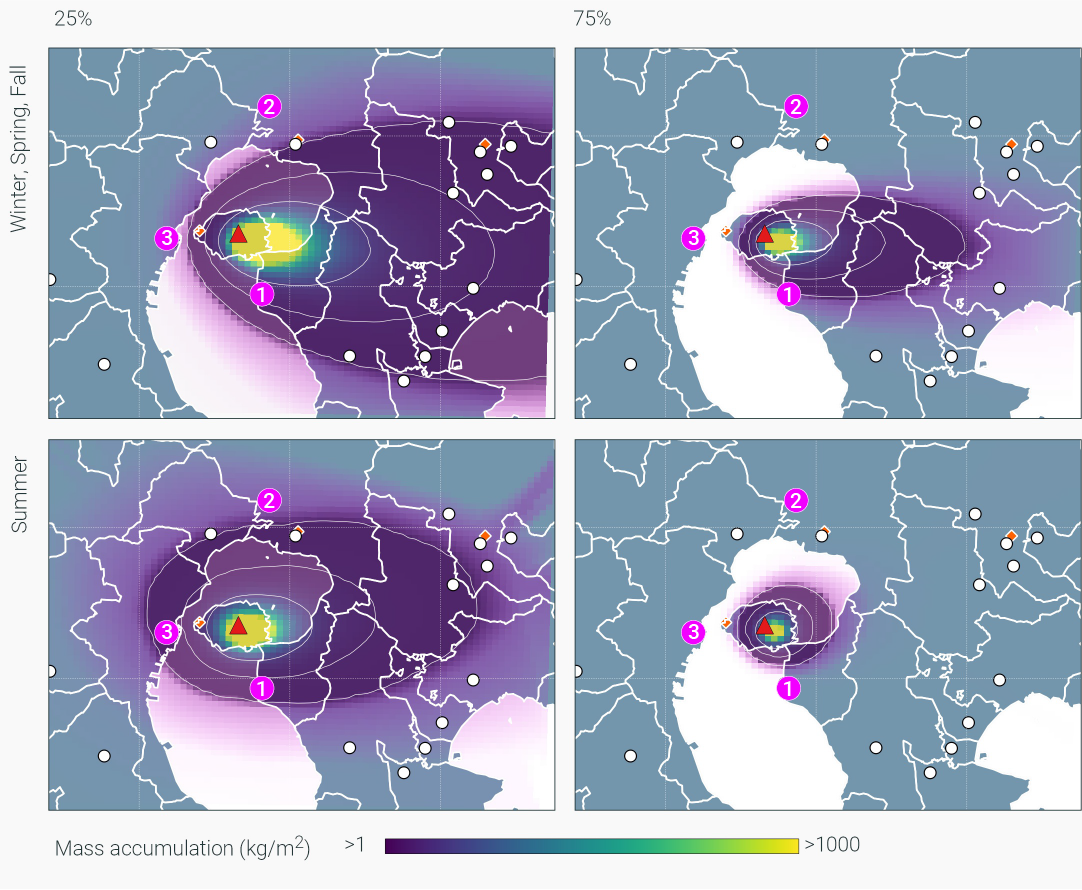
\includegraphics[width=.7\textwidth]{../docs/img/sakurajima/im.png}
    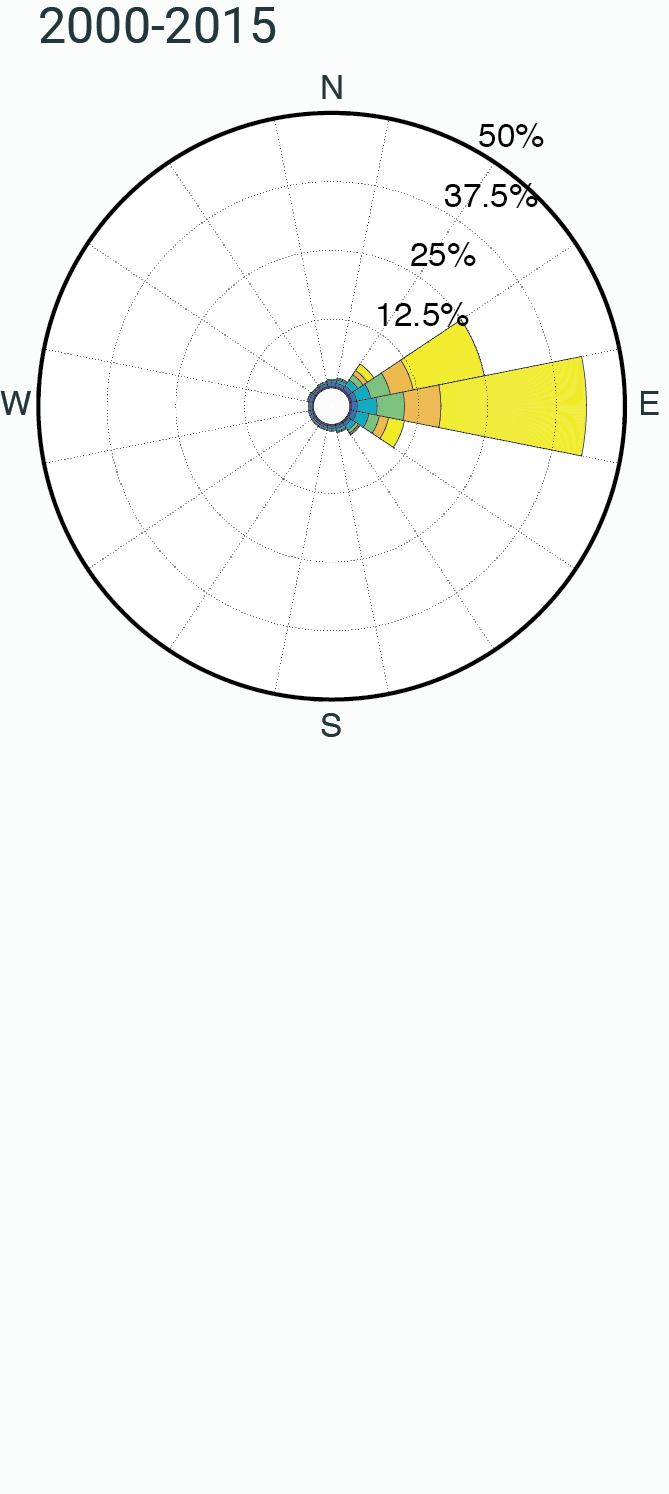
\includegraphics[width=.25\textwidth]{img/wind_all.png}
  }
\end{frame}


\begin{frame}{Probability $\rightarrow$ isomass maps}
  \only<1>{
    \centering 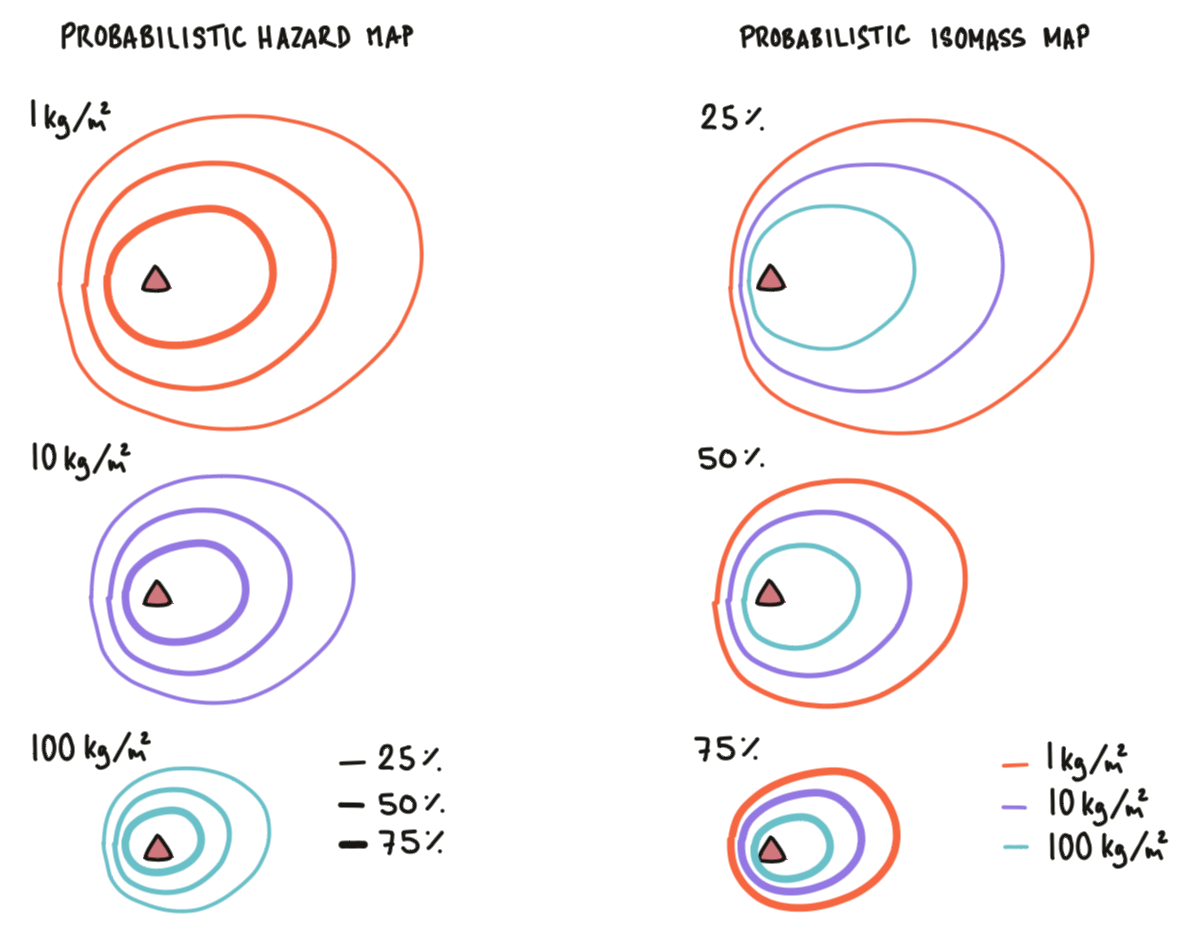
\includegraphics[width=.7\textwidth]{../docs/img/pim/prob2im1.png}
    }
  \only<2>{
    \centering 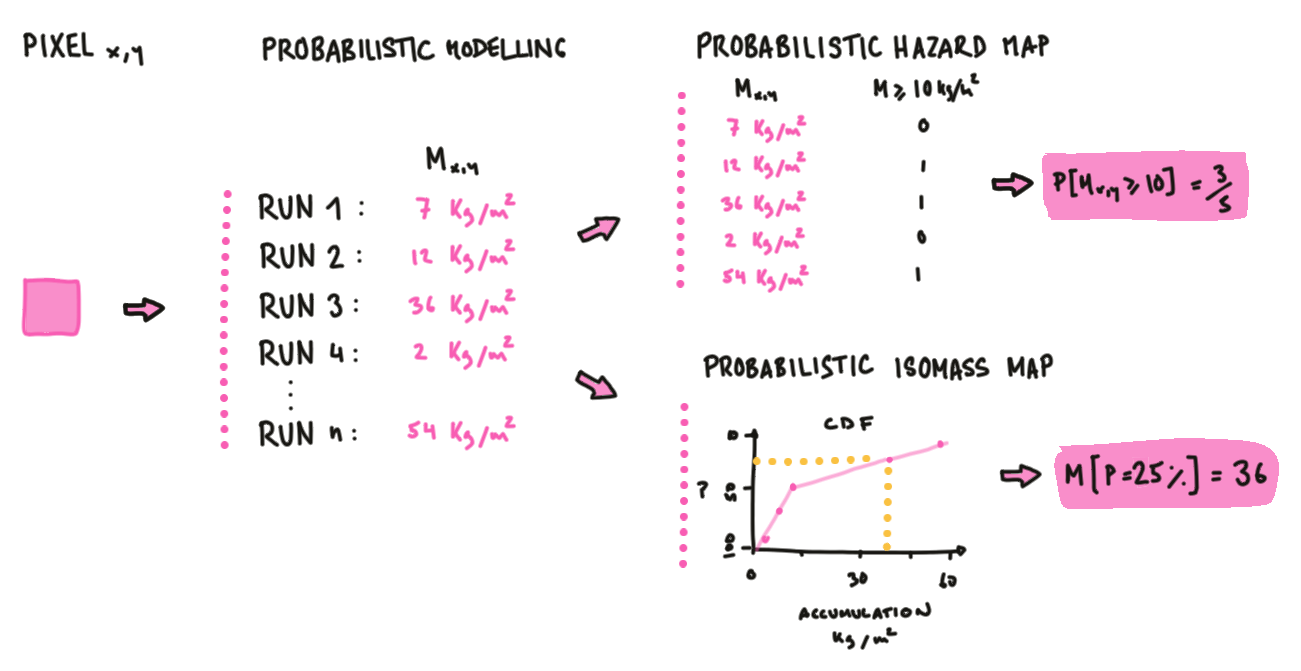
\includegraphics[width=1\textwidth]{../docs/img/pim/prob2im2.png}
  }
\end{frame}



\begin{frame}{Method 3: Hazard curves}
  \only<1>{
    \begin{columns}[T]
      \begin{column}{0.6\textwidth}	
        \textbf{Hazard curves}:\vspace*{1em}
        \begin{itemize}
          \item \alert{Fixed} latitude and longitude ($\rightarrow$ one point) \vspace*{1em}
          \item Other quantities are expressed \alert{continuously} \vspace*{1em}
          \item Display the probability of occurrence of a given tephra accumulation for a single location \vspace*{1em}
          \item There are \alert{as many curves} as points of interest \vspace*{1em}
        \end{itemize}
      \end{column}
      
      \begin{column}{0.4\textwidth}	
        \centering 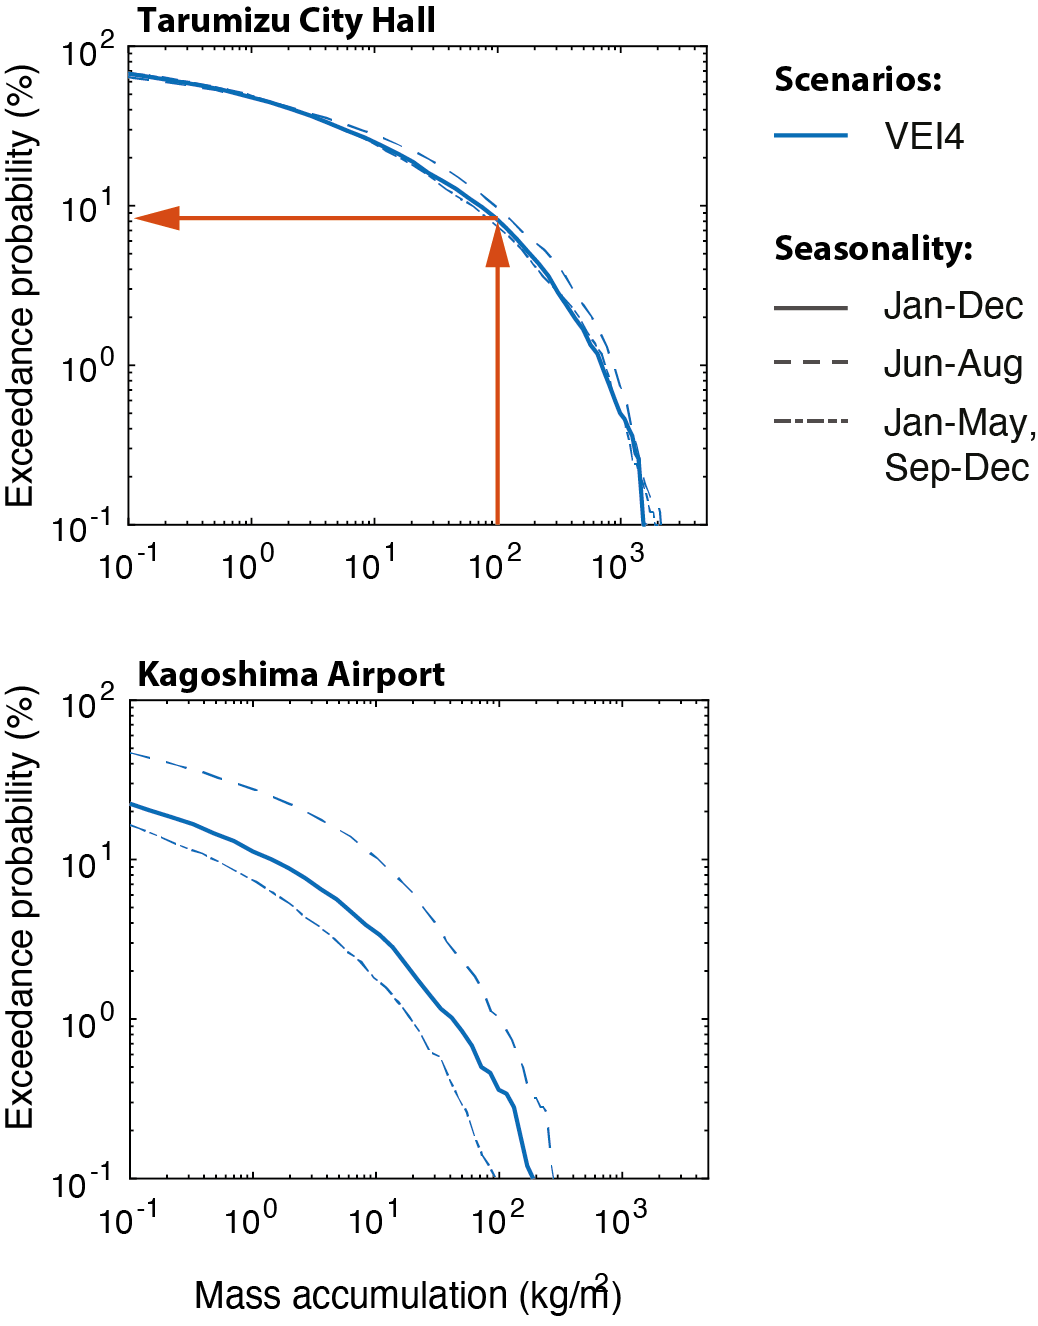
\includegraphics[width=1\textwidth]{img/curves.png}
      \end{column}
    \end{columns}
  }
\end{frame}


\begin{frame}[standout]
  \alert{Exercise:} Scenario--based probabilistic hazard assessment for tephra fallout for La Palma
\end{frame}



\begin{frame}[t]{Exercise}

    \begin{columns}[T]
      \begin{column}{0.6\textwidth}	
        \only<1->{  
          \textbf{Objectives:}
            \begin{itemize}
              \item Analyse the \alert{eruptive record}
              \item Analyse \alert{wind patterns} in a region
              \item Define an \alert{eruption scenario} and \alert{ESPs}
              \item Analyse \alert{hazard outputs}
            \end{itemize}
          }
          \only<2->{ 
            \textbf{Eruption scenario:}\\
            \begin{itemize}
              \item Low-intensity VEI 3 eruption 
              \item Similar volume, but long--lasting and less intense
            \end{itemize}
          }
          \only<3->{ 
            \textbf{Admin:}\\
            \begin{itemize}
              \item Produce \alert{hazard maps}
              \item Answer \alert{question sheet}
            \end{itemize}
          }
      \end{column}
      \begin{column}{0.4\textwidth}	
        
        \only<2>{
          Volcanic Explosivity Index (VEI) \\ \vspace*{1em}
          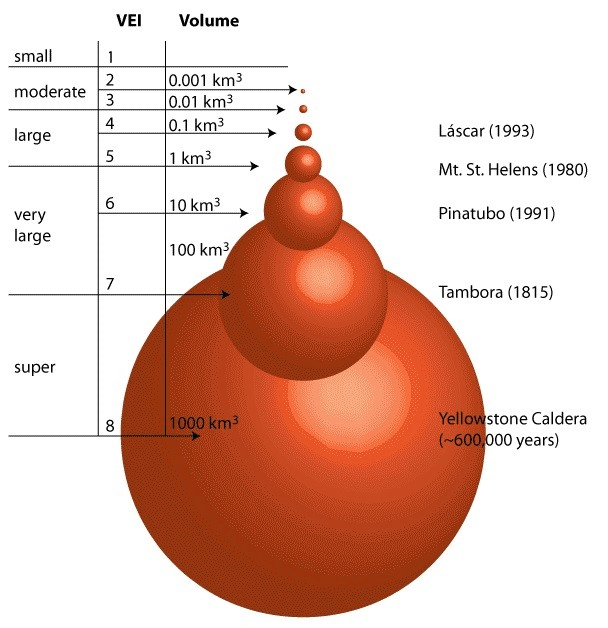
\includegraphics[width=1\textwidth]{../docs/img/tephra/vei.png}}
      \end{column}
    \end{columns}
\end{frame}


  % \centering \textbf{Uncertainties:}\\
  %   \vspace*{1em}
  %   $\rightarrow$ \alert{Epistemic uncertainties}: derives from the \alert{lack of knowledge} regarding a phenomena. In theory, we could reduce it with more \alert{knowledge}.\\ \vspace*{1em}
  %   $\rightarrow$ \alert{Aleatoric uncertainties}: associated with the inherent randomness of natural processes. Nothing much we can do about it, really!

  
  % \only<2>{
  %   \begin{columns}[T]
  %     \begin{column}{0.45\textwidth}	
  %       \textbf{ESP distributions}:\vspace*{1em}
  %       \begin{itemize}
  %         \item Account for both \alert{epistemic} and \alert{aleatory} uncertainties
  %         \item Reflect our \alert{knowledge} of the system
  %         \item Based on:
  %         \begin{itemize}
  %           \item[$\rightarrow$] Ideally, \alert{field studies} 
  %           \item[$\rightarrow$] \alert{Literature} reviews 
  %           \item[$\rightarrow$] \alert{Analogue} volcanoes/eruptions 
  %           \item[$\rightarrow$] Eruption \alert{databases}
  %         \end{itemize}
  %       \end{itemize}
        
  %     \end{column}
      
  %     \begin{column}{0.55\textwidth}	
        
  %       \centering 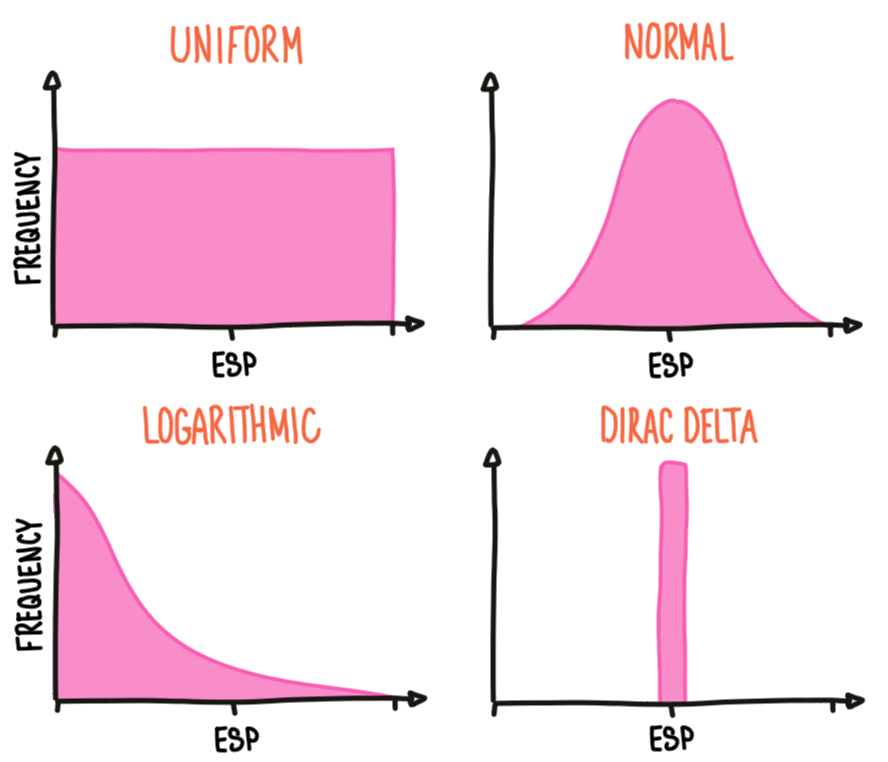
\includegraphics[width=1\textwidth]{../docs/img/ESP/ESP-distributions.png}
  %   \end{column}
  % \end{columns}
  % }
% \end{frame}


% \begin{frame}{Course's objectives \& schedule}
%   \only<1>{ \includegraphics[width=\textwidth]{Fig/workflow1.png} } 
%   \only<2>{

%     \begin{columns}[T] 
%       \begin{column}{0.5\textwidth}	
%         \textbf{Day 1: \alert{Lava flow}}        
%           \begin{enumerate}
%             \item Lava flow modeling using several approaches
%             \item Introduction to probabilistic hazard assessment
%             \item Hazard assessment of lava flows
%           \end{enumerate}
%       \end{column}

%       \begin{column}{0.5\textwidth}	
%         \textbf{Day 2: \alert{Tephra fallout}}        
%           \begin{enumerate}
%             \item Introduction to tephra fallouts and ESP
%             \item Deeper into probabilistic hazard assessment
%             \item Probabilistic hazard assessment for tephra fallout
%           \end{enumerate}
%       \end{column}
%     \end{columns}

    
%   } 
% \end{frame}

% \begin{frame}{Some admin}
%   \scriptsize
%   \begin{table}[htbp]
%     \centering
%       \begin{tabular}{llllr}
%       \textbf{\alert{Vent 1}} & \textbf{\alert{Vent 2}} & \textbf{\alert{Vent 3}} & \textbf{\alert{Vent 4}} & \textbf{\alert{Vent 5}} \\ 
%       Fernanda Naranjo Hidalgo & Camille Pastore & Monique Johnson & Million Mengesha & \multicolumn{1}{l}{Anabella Fantozzi} \\
%       Mattias Coullie & John Gallego Montoya & Angie Ramirez Huerta & Ana Maria Perez Hincapie & \multicolumn{1}{l}{Jonas Schranz} \\
%       Florent Keller & Karen Nicollet & Elise Cerutti & Génio Lay Da Silva & \multicolumn{1}{l}{Nicolas Serrano} \\
%       Salome Gogoladze & Douglas Stumpp & David Gutierrez Rivera & Sylvain Köhli & \multicolumn{1}{l}{Amin Abutaleb} \\
%       Elias Garcia Urquia & Mario Cifuentes Jacobs & Delair Ndibi Etoundi & Giorgi Merebashvili &  \\
%       \end{tabular}%
%     \label{tab:addlabel}%
%   \end{table}%
%   \vspace*{2em}
%   \normalsize
%     \centering Theory + lab $\rightarrow$ \alert{Part of the grade!} $\rightarrow$ See question sheet on Moodle
  
% \end{frame}

% % \begin{frame}[standout]
% %   Today: \alert{Lava flows}
% % \end{frame}

% \section{Today: \alert{Lava flows}}

% \begin{frame}{Lava flows}
%   \only<1>{ \centering \includegraphics[width=1\textwidth]{img/lava_flow.png} \\ \vspace*{1em}
%     Lava channel $\rightarrow$ A'a $\rightarrow$ Pahoehe \\  
%   }
% \end{frame}

% % - Lava flows -> infrastructures
% % - Hawaii, DRC, La Palma
% % - Slow moving, not lethal, but
% % - Long lasting crises, high uncertainties
% % - Complex phenomenon, can extend 10th of km from the source 
% % - Emergency management is complex, requires proper channels of communication between scientific institutions, decision makers, stakeholders

% \begin{frame}{Pahoa crisis, Hawaii, 2014}
%   \only<1>{ \centering \includegraphics[width=.55\textwidth]{img/HI.pdf} }
%   \only<2>{ \centering \includegraphics[width=1\textwidth]{img/pahoa.png} }
% \end{frame}

% % - Communication: Puhoho active since the 80's
% % - Repeated impacts on the community

% \section{\alert{Lava flow part I} \\Path of steepest descent}

% \begin{frame}[t]{Path of steepest descent}
%   \begin{columns}[T]
%     \begin{column}{0.5\textwidth}	
%       \only<1>{
%         \centering 
%         \textbf{DEM}: Digital Elevation Models \\
%         $\downarrow$ \\ 
%         \textbf{Hydrological models}  \\ 
%         $\downarrow$ \\ 
%         \texttt{Flow accumulation} $\rightarrow$ \texttt{Stream network} $\rightarrow$ \texttt{Drainage basins}
%       }
%       \only<2>{
%         \textbf{Flow accumulation}
%         \begin{itemize}
%           \item \alert{Cumulative number of upstream pixels that contribute to surface water drainage to any given downstream pixel}
%           \item From any pixel, flow goes in the direction of the \alert{largest} $-\Delta Z$
%           \item Once flow direction is estimated, the algorithm counts \alert{how many upstream pixels} contribute to any given downstream pixel
%         \end{itemize}
%       }
%       \only<3>{
%         \textbf{Stream network}
%         \begin{itemize}
%           \item Applies a threshold of count values $c$ to the \alert{Flow Accumulation} raster to delineate a \textbf{stream}
%           \item If a given pixel has a number of contributing pixels $C$ such as $C \geq c$, then the pixel is assumed to be part of the stream
%           \item \alert{Stream} network is a synonym of \alert{path of steepest descent}
%         \end{itemize}
%       }
%       \only<4>{
%         \textbf{Drainage basins}
%         \begin{itemize}
%           \item Classifies which stream each pixel contributes to. 
%           \item Think of it as a watershed, where ridges act as limits between zone contributing to different streams and valleys accumulate most of the surface flow.
%         \end{itemize}
%       }
%     \end{column}

%     \begin{column}{0.5\textwidth}	
%       \only<1>{
%         \includegraphics[width=1\textwidth]{../docs/img/hydro/hydro1.png}
%       }
%       \only<2>{
%         \includegraphics[width=1\textwidth]{../docs/img/hydro/hydro2.png}
%       }
%       \only<3>{
%         \includegraphics[width=1\textwidth]{../docs/img/hydro/hydro3.png}
%         }
%         \only<4>{
%         \includegraphics[width=1\textwidth]{../docs/img/hydro/hydro4.png}
%       }
%     \end{column}
%   \end{columns}
% \end{frame}

% \begin{frame}[standout]
%   \alert{Exercise 1:} Path of steepest descent for La Palma \\ \vspace*{1em}
% \end{frame}

% \begin{frame}[t]{Exercise 1: Path of steepest descent for La Palma}
  
%   \only<1-2>{
%     \textbf{Aims:}
%     \begin{itemize}
%       \item Analyse \alert{hydrological properties} of la Palma based on a 25-m DEM 
%       \item Revisit \alert{historical lava flows} based on the geological map
%       \item Get a \alert{critical} perspective on the path of steepest descent approach
%     \end{itemize} 
%   }

%   \only<2>{
%     \textbf{Workflow:}
%     \begin{itemize}
%       \item Go to http://cerg-c.github.io 
%       \item Go through the following exercises:
%       \begin{itemize}
%         \item \alert{Teaching / Setting up QGIS}
%         \item \alert{Teaching / Lava hazard / Introduction}
%         \item \alert{Teaching / Lava hazard / Getting started}
%         \item \alert{Teaching / Lava hazard / Steepest descent}
%       \end{itemize}
%     \end{itemize}
%     }
%   \only<4>{
%     \textbf{Don't forget} to fill up the \alert{questions sheet}!\\
%   }
%   \only<3->{
%     \vspace*{2em}
%     \textbf{Let's get started together}
%     \begin{enumerate}
%       \item Start \alert{QGIS}, change language
%       \item Install \alert{Q-LavHA}
%       \item \alert{Download} and \alert{load} QIS data
%     \end{enumerate}
%   }



%   \end{frame}


% \begin{frame}[standout]
%   How likely are you to recommend the \alert{path of steepest descent} to a friend?\\
%   $\star \star \star \star \star $
% \end{frame}

% \section{\alert{Lava flow part II} \\ Modeling lava flows}

% \begin{frame}{When and why do lava flows?}

%     \begin{columns}[T]
%       \begin{column}{0.65\textwidth}	

%         \only<1-2>{
%           \textbf{Shear stress}\\ \vspace*{.5em}
          
%           The shear stress $\tau$ is the \alert{load stress applied to a fluid} $\rightarrow$ i.e., the force per unit area acting in the direction and parallel to the flow surface:

%           $$ \tau = \rho g h \times sin(\alpha)\ [Pa = Nm^{-2}]  $$
%         }

%         \only<2>{
%           \textbf{Strain rate}\\ \vspace*{.5em}
%           The strain rate $\epsilon$ is the \alert{rate of deformation} when a shear stress is applied $\rightarrow$ i.e., velocity gradient:

%           $$ \epsilon = \frac{dV}{dZ}\ [s^{-1}] $$

%         }

%         \only<3-4>{
%           \textbf{Yield strength}\\ \vspace*{.5em}
          
%           The yield strength $\tau _0$ is the \alert{shear stress} above which deformation begins**:

%           $$\tau_0 = \rho g h_0 \times sin(\alpha)\ [Pa = Nm^{-2          }]$$
%         }

%         \only<4>{

%           \textbf{Viscosity}\\ \vspace*{.5em}

%           The viscosity $\eta$ is the \alert{resistance of fluid} to flow when shear stress is applied:

%           $$\eta = \frac{d\tau}{d\epsilon}\ [Pa\ s = Nm^{-2}          s]$$

%         }

%         \only<5>{
%           \textbf{Summary:}\\ \vspace*{.5em}
%           \begin{itemize}
%             \item Flow occurs when \textbf{driving forces} \alert{exceed} \textbf{resistive forces}
%             \item Response/behaviour of the fluid depends on its \textbf{rheology}
%           \end{itemize}
%         }

%       \end{column}

%       \begin{column}{0.35\textwidth}	
%         \includegraphics[width=1\textwidth]{img/rheology.png}
%       \end{column}
%     \end{columns}

    
% \end{frame}

% \begin{frame}{Flow types}

%     \begin{columns}[T]
%       \begin{column}{0.65\textwidth}	

%         \only<1-2>{
%           \textbf{Newtonian fluids}\\ \vspace*{.5em}
          
%           \begin{itemize}
%             \item Newtonian fluids start to flow/deform when an \alert{infinitesimally low shear stress is applied}
%             \item The relationship between the applied force ($\rightarrow$shear stress) and rate of deformation ($\rightarrow$strain rate) is \alert{linear}
%           \end{itemize}
          
%         }

%         \only<2>{
%           \textbf{Non-newtonian fluid}\\ \vspace*{.5em}
          
%           A fluid is non-newtonian when one of these conditions is met:
%           \begin{itemize}
%             \item The relationship between shear stress and strain rate is \alert{non-linear}
%             \item A \alert{yield strength must be exceeded} before flowing occurs, after which the shear stress/strain rate relationship can be linear or not
%           \end{itemize}
          
%         }

%         \only<3-4>{
%           \textbf{Non-newtonian fluid}\\ \vspace*{.5em}
          
%           Amongst non-newtonian fluids, fluids with variable shear stress/strain rate include:
%           \begin{itemize}
%             \item \textbf{Dilatant fluids}: apparent viscosity increases with increasing shear rate $\rightarrow$ \alert{shear thickening fluids}
%             % Cornstarch
%             \item \textbf{Pseudoplastic fluids}: apparent viscosity decreases with increasing shear rate $\rightarrow$ \alert{shear thinning fluids}
%             % Quicksand, ketchup
%           \end{itemize}
%         } 
%         \only<4>{
%           \vspace*{2em}
%           \textbf{Bingham fluids} are a special type of non-newtonian fluids characterized by a \alert{yield strength} and a \alert{linear shear stress/strain rate relationship}
%         }
%         % \only<5>{
          
%         %   \textbf{Lava flows:} \vspace*{2em}
%         %   \begin{itemize}
%         %     \item Non-newtonian
%         %     \item Pseudoplastic
%         %     \item Yield strength
%         %   \end{itemize}
%         % }

%       \end{column}

%       \begin{column}{0.35\textwidth}	
%         \includegraphics[width=1\textwidth]{img/rheology.png}
%       \end{column}
%     \end{columns}

    
% \end{frame}


% \begin{frame}[standout]
%   Experiment time!
% \end{frame}
 
% \begin{frame}[standout]
%   Movie time!
% \end{frame}

% \begin{frame}{Lava flow videos}
  
%   \textbf{Put these physical concepts in the perspective of actual lava flows!}\\
%   Look at these videos, and describe them in terms of:

%   \begin{itemize}
%     \item Flow \alert{shape}, \alert{geometry}, \alert{morphology}, \alert{texture}
%     \item \alert{Colour} (as an indicator to which physical parameter)
%     \item \alert{Velocity} and flow rate
%     \item \alert{Driving} and \alert{resisting} forces
%   \end{itemize} 
  
%   \vspace*{2em}
%   \textbf{What type of fluid are \alert{lava flows}?}
% \end{frame}


% \begin{frame}[standout]
%   \alert{Conclusion:} It is slightly more complicated...
% \end{frame}


% \begin{frame}{Case study: the 2016 61G flow}
  
%   \only<1>{ 
%     \begin{columns}[T]
%       \begin{column}{0.5\textwidth}	
%         \centering \includegraphics[width=1\textwidth]{../docs/img/61g/HI.png}
%       \end{column}

%       \begin{column}{0.5\textwidth}	
%         \centering \includegraphics[width=1\textwidth]{../docs/img/61g/61g.jpg}
%       \end{column}
%     \end{columns}
%   }
%   \only<2>{
%     \centering Pahoehoe toes $\rightarrow$ \alert{Thermal insulation} $\rightarrow$ Lava tube
%     \begin{columns}[T]
%       \begin{column}{0.5\textwidth}	
%         \centering \includegraphics[width=.8\textwidth]{../docs/img/61g/toes.png}
%       \end{column}

%       \begin{column}{0.5\textwidth}	
%         \centering \includegraphics[width=.8\textwidth]{../docs/img/61g/tube.png}
%       \end{column}
%     \end{columns}
%   }
%   \only<3>{
%     \centering Morphology transition $\rightarrow$ \alert{Topography}
%     \includegraphics[width=.8\textwidth]{../docs/img/61g/pali.png}
%   }
%   \only<4>{
%     \centering Structure-from-motion $\rightarrow$ \alert{DEM evolution}\vspace*{.8em}
%     \includegraphics[width=.8\textwidth]{../docs/img/61g/DEM.png}
%     }
%   \only<5>{
%     \centering DEM evolution $\rightarrow$ \alert{Validation of steepest descent}\vspace*{.8em}
%     \includegraphics[width=.9\textwidth]{../docs/img/61g/steepest.png}
%   }
%   \only<6>{
%     \centering Thermal imagery $\rightarrow$ \alert{Heat budget}\vspace*{.8em}
%     \includegraphics[width=1\textwidth]{../docs/img/61g/thermal.png}
%   }
% \end{frame}


% \begin{frame}{Perspective}
%   \only<1>{
%     Lava flows often result in \alert{long--lasting crises} characterised by \alert{large uncertainties}. This is partly the case because:
%     \begin{itemize}
%       \item Lava flows are \alert{too complex} to (currently) be fully described by physical models 
%       \begin{itemize}
%         \item[$\rightarrow$] Spatio-temporal evolution of parameters affecting rheology,
%         \item[$\rightarrow$] Interaction with environment, stochastic processes
%       \end{itemize}
%       \item Need a framework to \alert{account for}, \alert{quantify} and \alert{communicate} \textbf{uncertainties}
%       \begin{itemize}
%         \item[$\rightarrow$] \alert{Epistemic} vs \alert{aleatory}
%       \end{itemize}
%     \end{itemize}
%     }
%   \only<2>{
%     \centering \alert{\textit{"A simple, imperfect model is better than no model"}}\\ \vspace*{1em}
%     \centering \alert{\textit{"All models are wrong, but some are useful"}}\\ \vspace*{1em}

%     \centering \begin{itemize}
%       \item[$\rightarrow$] A lot of models are available (see \alert{Resources} page) \textbf{but}
%       \item[$\rightarrow$] They require understanding \alert{limitations} and \alert{sources of uncertainties}
%     \end{itemize}
%   }

% \end{frame}

% \section{\alert{Lava flow part III} \\ Probabilistic modeling}

% \begin{frame}{Vent location}
%     \begin{columns}[T]
%       \begin{column}{0.5\textwidth}	
%         \centering \textbf{Monogenetic vents}\\ \vspace*{1em}
%         \centering\includegraphics[width=.85\textwidth]{img/lapalma.png}
%       \end{column}

%       \only<1>{
%       \begin{column}{0.5\textwidth}	
%         \centering \textbf{Future eruptions}\\ \vspace*{1em}
%         \centering\includegraphics[width=.55\textwidth]{../docs/img/hydro/Marrero_vents.png}
%       \end{column}
%       }
%       \only<2>{
%       \begin{column}{0.5\textwidth}	
%         \centering \textbf{Multiple vents for one eruptions}\\ \vspace*{1em}
%         \centering\includegraphics[width=.85\textwidth]{img/lapalma_2.png}
%       \end{column}
%       }
%     \end{columns}
%  \end{frame}

% \begin{frame}[standout]
%   How do we account for the \alert{uncertainty on vent location} in our hazard assessment for lava flow inundation?
% \end{frame}

% \begin{frame}[t]{Exploring vent location...}
%   ...using a frequentist approach:
%   \begin{columns}[T]
%     \begin{column}{0.5\textwidth}
      
%       \begin{enumerate}
%         \item<1- | alert@1> Assumption that a new vent can open from all these vents
%         \begin{itemize}
%           \item[$\rightarrow$]<1-> For now, assume \textit{equal probability}
%         \end{itemize}
%         \item<2- | alert@2> Run \textit{path of steepest descent} from all vents
%         \begin{itemize}
%           \item[$\rightarrow$]<2-> Some pixels are \textit{more likely} to be inundated
%         \end{itemize}
%         \item<3- | alert@3> Count the \textbf{number of times} a given pixel is inundated and \textbf{normalise} by the number of vents
%       \end{enumerate}

%     \end{column}

%     \begin{column}{0.5\textwidth}	
%       \only<1>{
%         \includegraphics[width=1\textwidth]{../docs/img/hydro/prob1.png}
%       }
%       \only<2>{
%         \includegraphics[width=1\textwidth]{../docs/img/hydro/prob2.png}
%       }
%       \only<3>{
%         \includegraphics[width=1\textwidth]{../docs/img/hydro/prob3.png}
%       }
%     \end{column}
%   \end{columns}
% \end{frame}

% \begin{frame}[t]{Deterministic vs probabilistic modeling}
%   \only<1-2>{
%   \begin{columns}[T]
%     \begin{column}{0.5\textwidth}
      
%       \only<1>{
%         \centering \textbf{Deterministic scenario}\\ \vspace*{1.2em}

%         \centering 
%         \alert{One} user-defined value for each model input \\
%         $\downarrow$\\
%         \alert{One} model run\\
%         $\downarrow$\\
%         \alert{One} possible outcome
%       }

%       \only<2>{
%         \centering \textbf{Probabilistic scenario}\\ \vspace*{1.2em}

%         \centering 
%         \alert{Range} of values as model inputs \\
%         $\downarrow$\\
%         \alert{Many model runs} with input conditions \alert{sampled} in input ranges\\
%         $\downarrow$\\
%         Aggregation of \alert{all possible outcomes} into \alert{probabilities}\\ \vspace*{.8em}
%         $\downarrow$\\ \vspace*{.8em}
%         \textbf{Allows exploring:}\\
%         $\rightarrow$ \alert{Uncertainties} on input parameters\\
%         $\rightarrow$ What \alert{could} happen in the future
%       }

%     \end{column}

%     \begin{column}{0.5\textwidth}	
%       \only<1>{
%        \centering \includegraphics[width=.575\textwidth]{img/lava_dt.png}
%       }
%       \only<2>{
%        \centering \includegraphics[width=.575\textwidth]{img/lava_prob.png}
%       }

%     \end{column}
%   \end{columns}
%   }
%   \only<3>{
%     \centering \includegraphics[width=.9\textwidth]{../docs/img/prob/prob1_wf.jpeg}
%   }


% \end{frame}


% \section{\alert{Lava flow part IV} \\ Q-LavHA}

% \begin{frame}{Q-LavHA}
%     \begin{columns}[T]
%       \begin{column}{0.5\textwidth}	
%         \begin{itemize}
%           \item<1- | alert@1> \textbf{Q-LavHA} $\rightarrow$ QGIS plugin
%           \item<1- | alert@1> Starting point $\rightarrow$ path of steepest descent
%           \item<2- | alert@2> Probabilistic approach to simulate:
%           \begin{itemize}
%             \item Flow \alert{inflation} $\rightarrow$ \alert{filling} depressions $\rightarrow$ lateral \alert{spreading}
%             \item Uncertainty on \alert{vent location}
%           \end{itemize}
%           \item<3- | alert@3> \alert{Thousands} of iteration of the path of steepest descent
%           \begin{itemize}
%             \item Next inundated pixel not only based on $\vert \Delta Z\vert $, but on a probability function based on $\vert \Delta Z\vert $ of all adjacent pixels
%           \end{itemize}
%           \item<4- | alert@4> \textbf{Output:} probability of flow inundation

%         \end{itemize}
%       \end{column}

%       \begin{column}{0.5\textwidth}	
%         \centering\includegraphics[width=1\textwidth]{img/qlavha_pixels.png}
%       \end{column}

%     \end{columns}
%  \end{frame}



% \begin{frame}[standout]
%   \alert{Exercise 2:} Probabilistic lava flow inundation hazard assessment for La Palma
% \end{frame}

% \begin{frame}[t]{Exercise 2: Probabilistic lava flow inundation hazard assessment}
%   \textbf{Aims:}
%   \begin{itemize}
%     \item Perform a probabilistic hazard assessment for lava flow inundation for La Palma
%     \item Contrast results when using \alert{point} vs \alert{surface} source
%   \end{itemize}
  
%   \only<2>{
%     \vspace*{1em}\textbf{Workflow:}
%     \begin{itemize}
%       \item Make sure you have installed \textbf{Q-LavHA}
%       \item Go through the \alert{Q-LavHA} exercise on http://cerg-c.github.io
%     \end{itemize}
%   }

%   \only<3>{
%     \vspace*{1em}\textbf{Don't forget:}
%     \begin{itemize}
%       \item To answer questions!
%     \end{itemize}
%   }
% \end{frame}


% \begin{frame}[standout]
%   \usebeamercolor[mWhite]{normal text}
%   Questions?\vspace*{.3cm}\\
%   \footnotesize \includegraphics[height=.2cm]{iconMail.pdf} \textmd{     sebastien.biasse@unige.ch}\\
%   \footnotesize \includegraphics[height=.25cm]{iconGit.pdf} \textmd{     e5k / http://e5k.github.io }
% \end{frame}


\end{document}







